% 美赛模板:正文部分

\documentclass[12pt]{article}  % 官方要求字号不小于 12 号,此处选择 12 号字体
% \linespread{1.1}
% \bibliographystyle{plain}
% 本模板不需要填写年份,以当前电脑时间自动生成
% 请在以下的方括号中填写队伍控制号
\usepackage[2107542]{easymcm}  % 载入 EasyMCM 模板文件
\problem{C}  % 请在此处填写题号
% \usepackage{mathptmx}  % 这是 Times 字体,中规中矩 
\usepackage{palatino}  % mathpazo 这palatino是 COMAP 官方杂志采用的更好看的 Palatino 字体,可替代以上的 mathptmx 宏包
\usepackage{pdfpages}
\usepackage{longtable}
\usepackage{tabu}
\usepackage{threeparttable}
\usepackage{listings}
\usepackage{paralist}
\usepackage{setspace}


 \let\itemize\compactitem
 \let\enditemize\endcompactitem
% \let\enumerate\compactenum
% \let\endenumerate\endcompactenum
% \let\description\compactdesc
% \let\enddescription\endcompactdesc
% \usepackage{biblatex} 
% \usepackage{cite}
% \usepackage{natbib}
\newcommand{\upcite}[1]{\textsuperscript{\textsuperscript{\cite{#1}}}}
\title{A Glimpse of Music Change through Influence Networks}  % 标题

% 如需要修改题头(默认为 MCM/ICM),请使用以下命令(此处修改为 MCM)
%\renewcommand{\contest}{MCM}

% 文档开始
\begin{document}
\begin{abstract}
	
	% (Need to be reviewed)
	Music is the treasure of humanity. The interplay of artists and genres has also contributed to the continuous development of music. The purpose of this paper is to develop a model for measuring musical influence and to explore the evolutionary and revolutionary trends in examining artists and genres.
	
	In \textsc{Task 1}, we treat each artist as a node and represent the node-to-node influence with a directed line segment. Then we quantify the direct influence by adapting the TwitterRank model and quantify the indirect influence by constructing a transmission of indirect influence modeled after \textit{Markov chains}. Finally, by studying the influence of individual nodes in a sub-network, we reveal the important people in this sub-network.
	

	
	% Here is the abstract of your paper.
	
	% Firstly, that is ...
	
	% Secondly, that is ...
	
	% Finally, that is ...
	
	% 美赛论文中无需注明关键字。若您一定要使用,
	% 请将以下两行的注释号 '%' 去除,以使其生效
	\vspace{5pt}
	\textbf{Keywords}: Markov chains, Random forest algorithm, Hierarchical clustering 
	
\end{abstract}
    
\maketitle  % 生成 Summary Sheet

\tableofcontents




% 正文开始
% Chapter 1: Introduction
\section{Introduction}

\subsection{Problem Background}
Music has been part of human societies since the beginning of time as an essential component of cultural heritage. There are many factors that can influence an artist's music making, especially between artists. The Integrative Collective Music (ICM) Society has asked our team to develop a model that measures musical influence, examining evolutionary and revolutionary trends of artists and genres.
The team are provided with the following tasks:

\begin{itemize}
	\setlength{\parsep}{0ex} %段落间距
	\setlength{\topsep}{2ex} %列表到上下文的垂直距离
	\setlength{\itemsep}{1ex} %条目间距
	\item Create a targeted music impact network and develop parameters to capture "music impact" in this network, describing what the "music impact" metrics reveal.
	\item Develop a music similarity metric. Use metrics to explore similarities between artists of the same genre and artists of different genres.
	\item Compare the similarities and influences between genres, explore the differences between genres, trends in genres over time, and the extent to which genres are related to each other.
	\item Explain whether the similarity data indicate that the identified influencers actually influence the respective artists, and explore whether the influencers have a wholesale or local influence on the followers.
	\item Identify the features that mark a major leap in the evolution of music and the influencers of major changes.
	\item Analyze the influential process of musical evolution of a genre over time, revealing indicators of dynamic influences and explaining how the genre or artist has changed over time.
	\item Expresses the influence of music in time or environment and the impact of social, political or technological change on music.
\end{itemize}

\subsection{Our work}

\begin{enumerate}[\bfseries 1.]
	\setlength{\parsep}{0ex} %段落间距
	\setlength{\topsep}{2ex} %列表到上下文的垂直距离
	\setlength{\itemsep}{1ex} %条目间距
	\item We treat each artist as a node and represent the node-to-node influence with a directed line segment. Then we quantify the direct influence by adapting the TwitterRank model and quantify the indirect influence by constructing a transmission of indirect influence modeled after \textit{Markov chains}. Finally, by studying the influence of individual nodes in a sub-network, we reveal the important people in this sub-network. 
	\item We use the \textit{random forest algorithm} to reduce the dimensionality of the features of artists' works, then vectorize each feature of artists' works, followed by using min-max to normalize the feature values, and then measure the similarity between artists by the \textit{cosine similarity}. Finally, we use \textit{hierarchical clustering method} to analyze the correlation between artists.
	\item We analyzed the correlations and influences between and within genres, using the Easy Listening genre as an example, in combination with the relationships of influence, and the degree of similarity. Based on this, we then identified the main characteristics of all genre styles.
	\item Using the artist Al Di Meola as an example, we analyzed the relationship between influence and the degree of similarity of the works in relation to the influence model we developed, and developed further analysis based on each of these characteristics.
	\item Using the folk genre as an entry point, we analyzed the change curve of each of its characteristic attributes over time, searched for curve inflection points, and identified the influencers of major changes using the similarity metric.
	\item We defined dynamic indicators of stylistic evolution based on similarity indicators and selected the Vocal genre to analyze in detail the influential process of its musical evolution over time. The artist Frank Sinatra from the Vocal genre is also used as an example to explain the reasons for the stylistic changes of his works over time.
	\item Combined with other sources, we analyzed the specific impact of environmental and temporal factors on music from four perspectives: political, economic, warfare, and technological.
\end{enumerate}


% \section{Introduction}
% \subsection{Problem Background}
% Here is the problem background ...

% Two major problems are discussed in this paper, which are:
% \begin{itemize}
%     \item Doing the first thing.
%     \item Doing the second thing.
% \end{itemize}

% \subsection{Literature Review}
% A literatrue\cite{1} say something about this problem ...

% \subsection{Our work}
% We do such things ...

% \begin{enumerate}[\bfseries 1.]
%     \item We do ...
%     \item We do ...
%     \item We do ...
% \end{enumerate}

% Chapter 2: 模型准备
\section{Assumptions and Notations}
\subsection{Assumptions}
\begin{itemize}
	\setlength{\parsep}{0ex} %段落间距
	\setlength{\topsep}{2ex} %列表到上下文的垂直距离
	\setlength{\itemsep}{1ex} %条目间距
	\item The relationship of influence between artists is related to their works, not their lives.
	\item The same artist can only belong to one genre. 
	\item The relationship of influence between artists is credible and real. 
	\item The effect between genres is considered only for the genre given in the data and does not include other genres.  
\end{itemize}

\subsection{Notations}
\begin{table}[H]
	\centering
	\begin{tabular}{ll}
		\hline
		\hline
		\multicolumn{1}{c}{\textbf{Notations}} & \textbf{Definition}\\ \hline
		$p_{ij}$                      & the direct influence from $i$ to $j$                      \\
		$q_{nn+2}$                      & the indirect influence from n to n+1                      \\
		$\mathcal{P}$                       & the attenuation degree of the influence                      \\
		$\eta$                      & the effective quantity for information                      \\
		$Inf_{i}$                      & the music influence of $i$                      \\
		$C_{ij}$                      & the similarity between $i$ and $j$                      \\
		$\varphi _(t)$                      &  Variance of similarity over time                     \\
		$\psi _(t)$                      & Activity changes with time                     \\
		$d_{ij}$                      & distence between $i$ and $j$                      \\                     
		\hline
		\hline
	\end{tabular}
	\caption{Notations Table}
\end{table}
\section{Task1: Network Model}
\subsection{Network for influence}

By observing the data, we find that each piece of data often contains several parts. The first is the unique ID of the influencer and the ID of the followers. So for these $n$ authors, we can use an $n\times n$ matrix to record the influence relationships between them.
\begin{equation}
\begin{pmatrix}
a_{11}&a_{12}&\cdots&a_{1n}\\
a_{21}&a_{22}&\cdots&a_{2n}\\
\vdots&\vdots&\ddots&\vdots\\
a_{n1}&a_{n2}&\cdots&a_{nn}\\
\end{pmatrix}
\end{equation}
Where the value of $a_{ij}$ is 1 or 0, indicating whether the author $i$ has influence on the author $j$, respectively. 

So from this matrix we can generate a network. We use nodes to represent each writer. Directed line segments are used to indicate that one node has a relationship to another node.
We also use different colors to indicate the different schools that writers belong to.

We randomly selected a few authors to generate the following network as a schematic:

\begin{figure}[H]
	\centering    
	\subfigure[organization1]{				% 图片1([]内为子图标题)
		\label{fig:sub.roomhot}							% 子图1的标签
		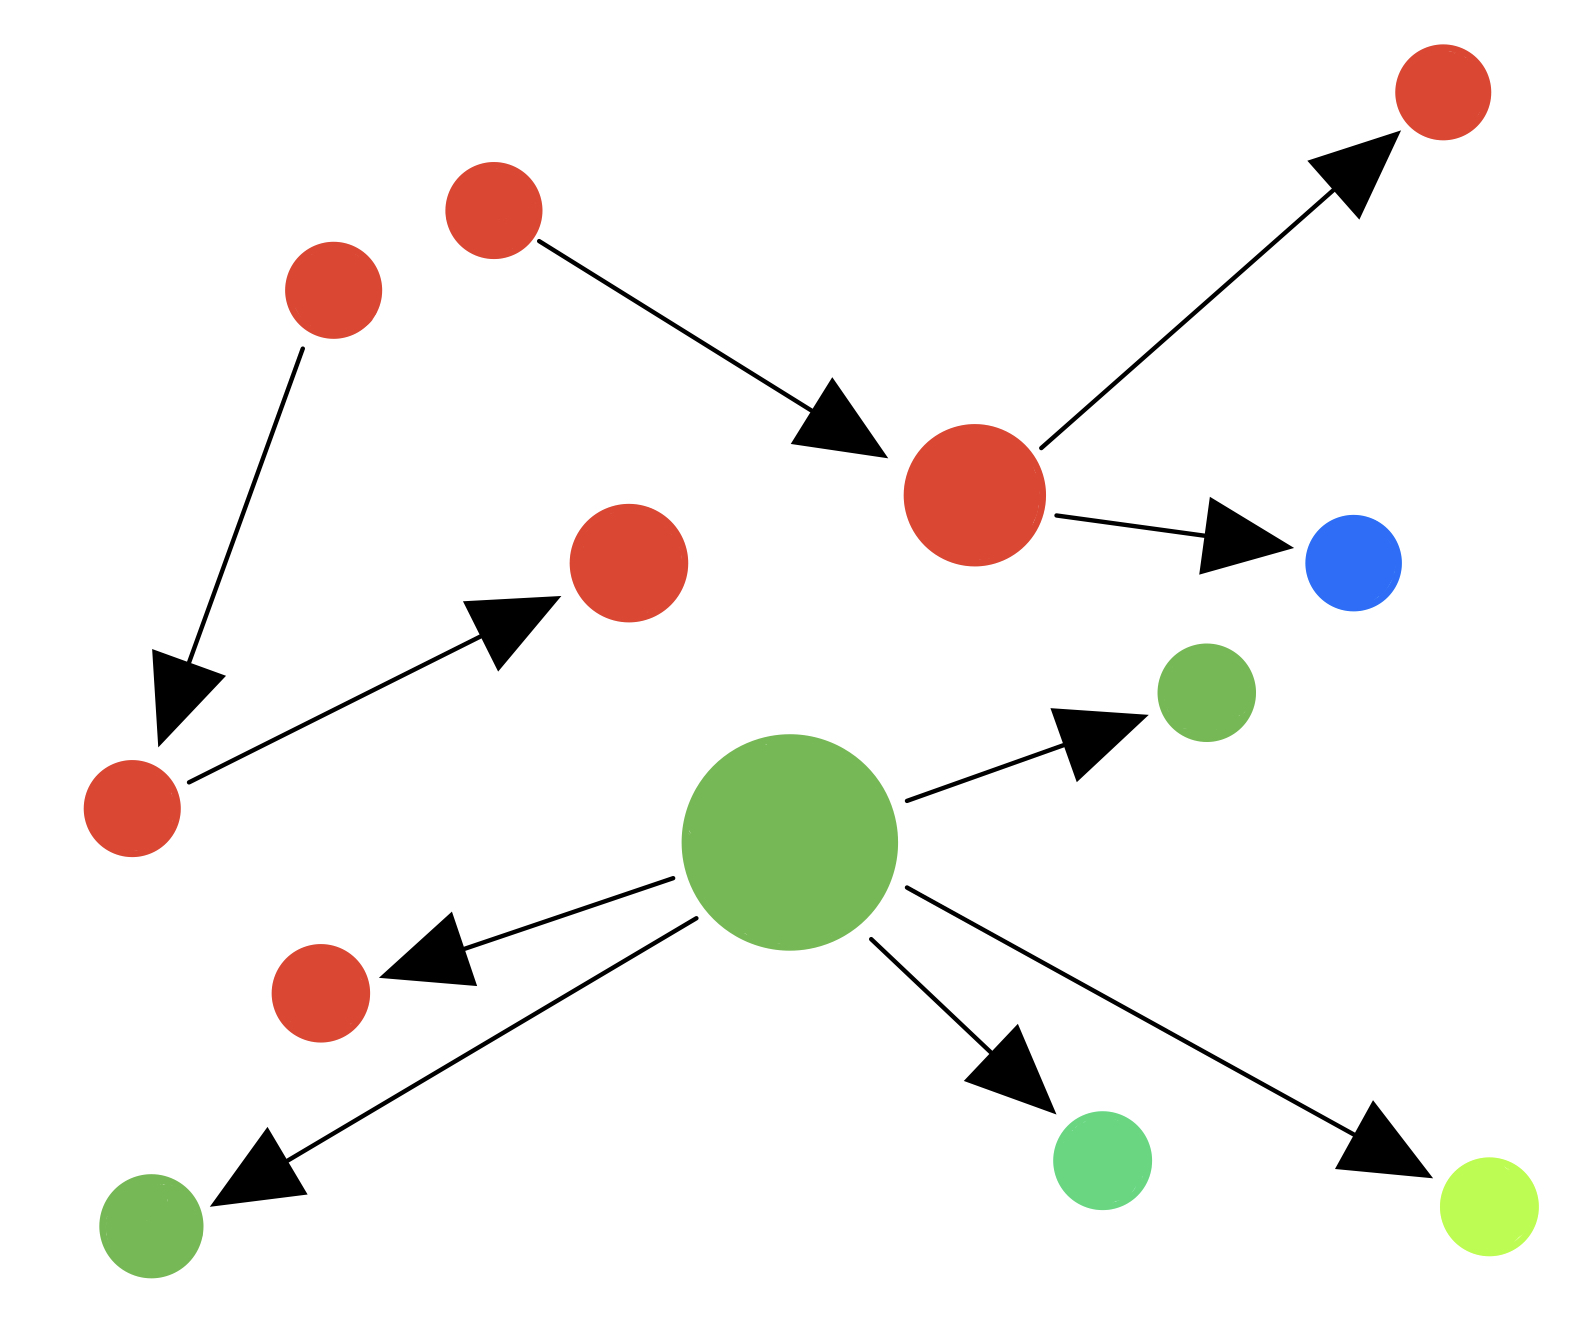
\includegraphics[width=0.3\textwidth]{network1.png}}% 子图1的相对位置
	\subfigure[organization2]{				% 图片2
		\label{fig:sub.floorhot}						% 子图2的标签
		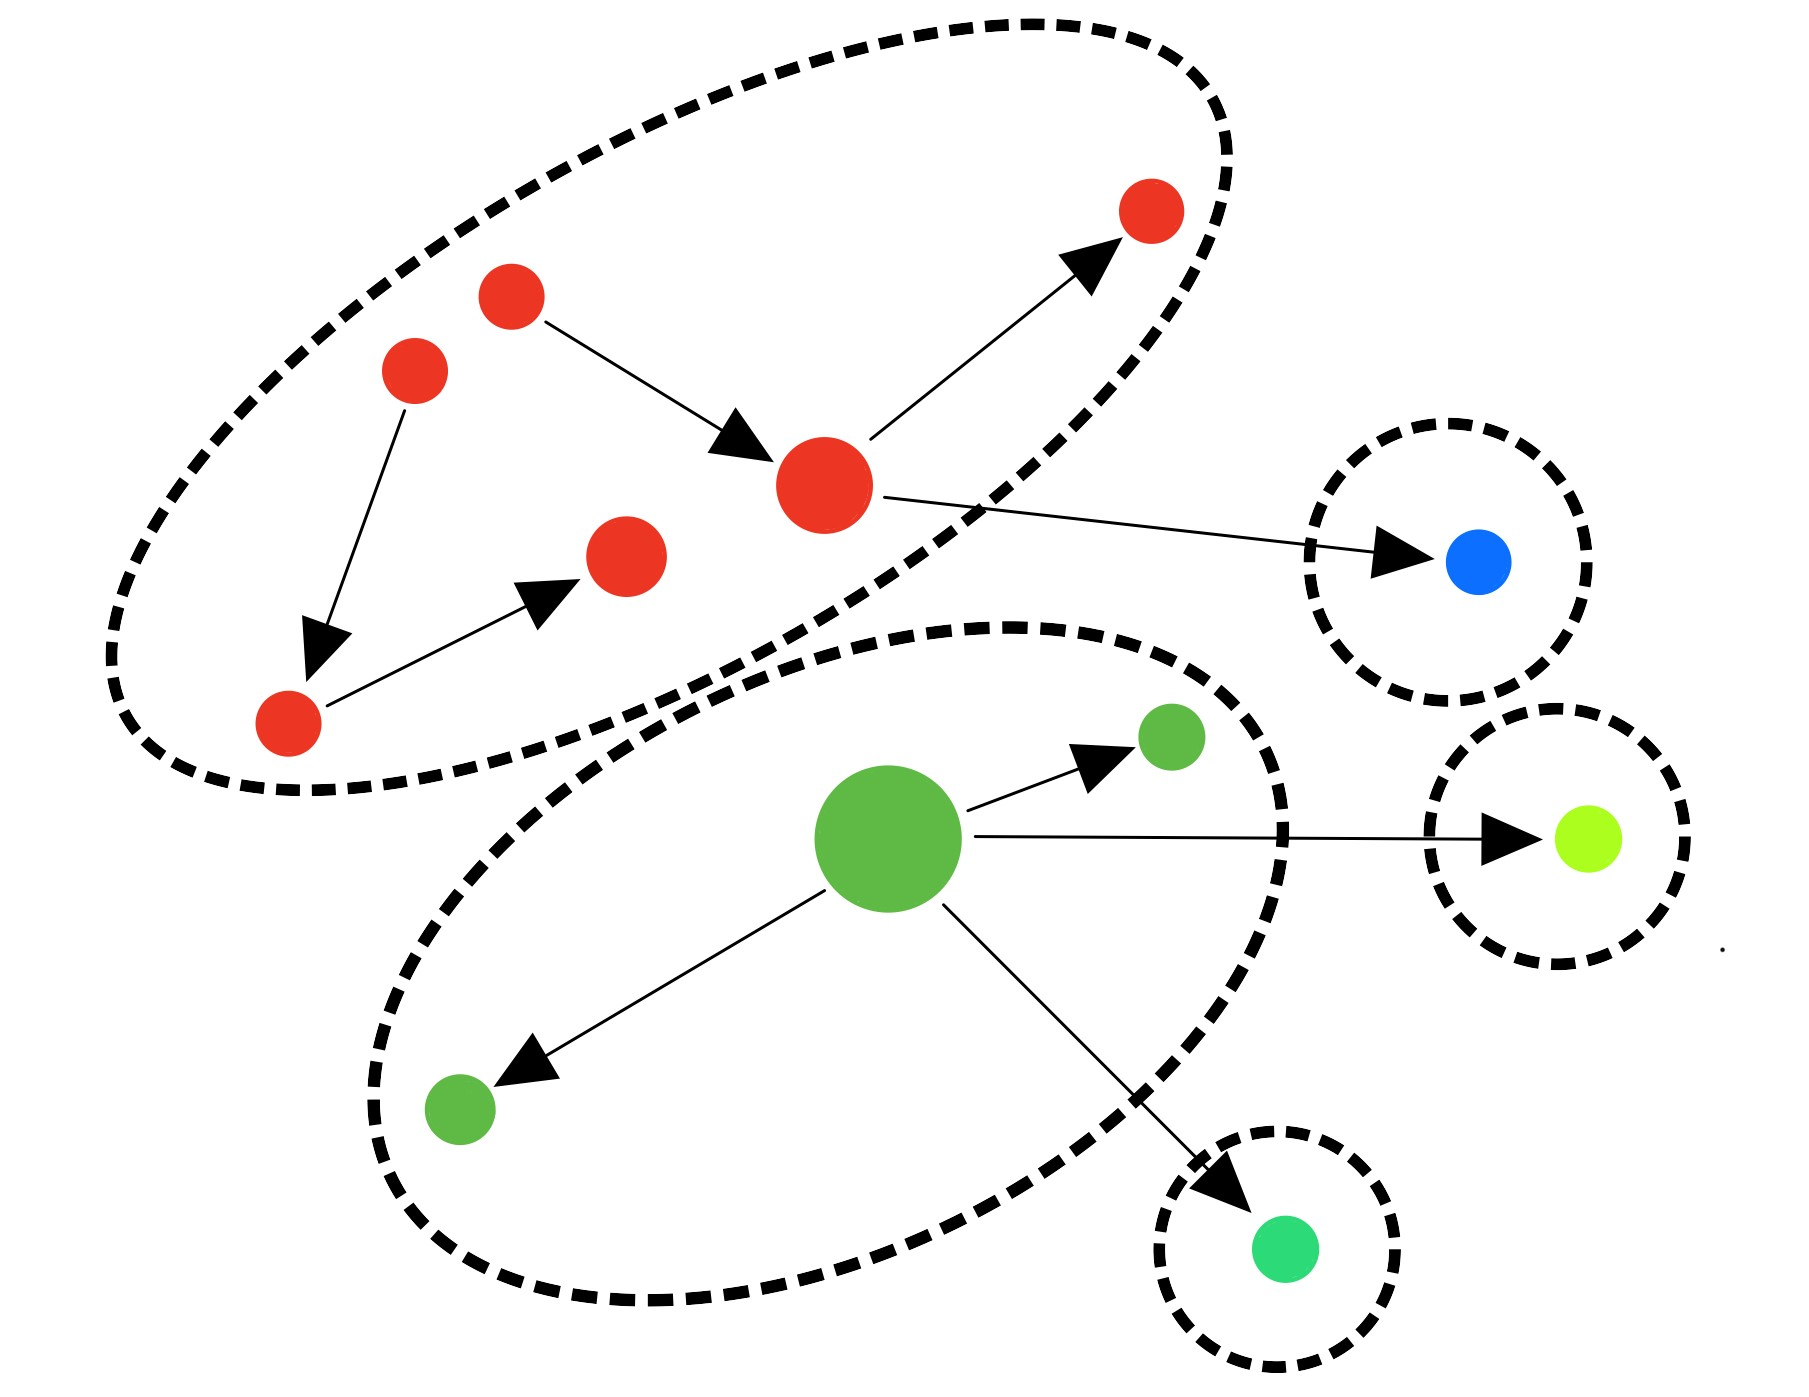
\includegraphics[width=0.3\textwidth]{organization.png}}% 子图2的相对位置
	\caption{Organization}		% 总图标题
	\label{fig:hot}									% 总图标签
\end{figure}


By combining all the artists' information into a matrix and generating a network, we will have a vast and complex network. In order to better analyze the network, we integrated our network into blocks, imitating the concept of community in complex network theory. Community structure defines a group of nodes in the network that are closely connected internally and sparsely connected externally as a community. These nodes usually have the same attributes or similar functions. Then in our network, we can artificially define a group of nodes belonging to artists of the same genre as a community.

The schematic diagram is as figure1(b):

Obviously, the community structure of this network is non overlapping, that is, each node can only belong to one community. This is a very important point. Through this point, we can use a larger node to replace the community, so that we can more intuitively observe the whole network. At the same time, we make the thickness of the directed line segment from node a to node B proportional to the number of small nodes in node A that affect the small nodes in node B.

In this way, we get a network graph based on all the data. Through this network graph, we can intuitively see the relationship between different communities and the important position of a community in the whole music field.

\begin{figure}[H]
	\centering
	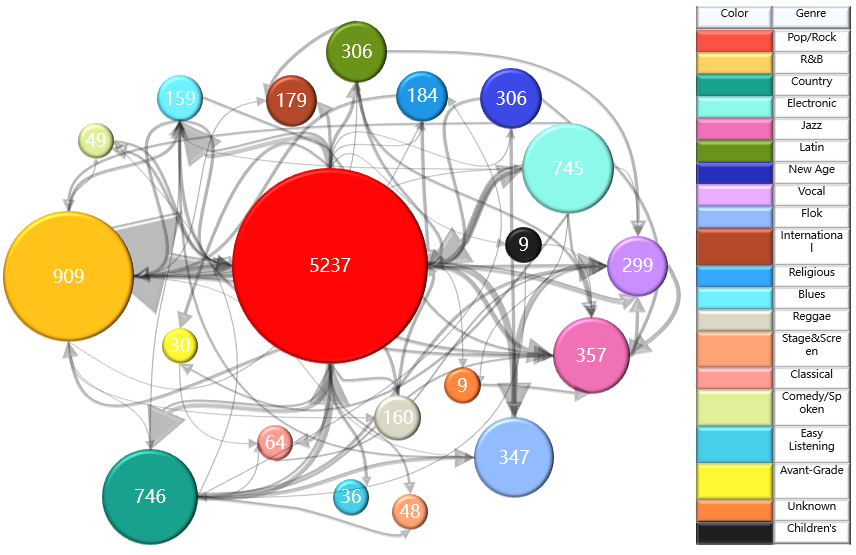
\includegraphics[width=.6\textwidth]{all network.png}
	\caption{network for all the nods at the community level}
	\label{img}
\end{figure}

From this, we can roughly observe that pop, R\&B, country and electronic play an important role in the whole history of music development.

\subsection{Music influence}
\subsubsection{Direct influence}

The influence of nodes in the network has been studied for a long time. Many scholars such as singla and Goyal\upcite{1} define the influence as the similarity and correlation between nodes. However, based on the data given in influence date, we can not understand the similarity between artists. The only similarity is whether these artists belong to the same school, that is, whether these nodes belong to the same community. Therefore, we introduce the twitterrank model proposed by Jianshu Weng:
\begin{equation}
p_{ij}=\frac{| T_j|  }{\Sigma_{\alpha : \text{i follows $\alpha$} } T_{j}}\cdot sim_{ij} 
\end{equation}
It's the influence of user i on user j. It should be noted that this model is proposed to study the influence among users in social networks. So we only need to understand its general idea, in which $sim$ represents the similarity between users. The first item on the right of the equation expresses the degree of difficulty that the message sent by the influencer is accepted by the follower.
Based on the communication theory of community network structure, a piece of information is easier to spread within a community. At the same time, for nodes in the same community, they should have higher similarity. In order to determine the similarity between the two, we use entropy weight method to make a simple comparison: The similarity of same organization is 0.6337, The similarity of different organization is 0.3662.

According to the information obtained, it is determined that the $sim$ between two nodes belonging to the same community is 0.63, while the $sim$ between two nodes in different communities is 0.36.

Then we determine the first term on the right side of the equation, because a piece of information is more easily spread within a community, so it has a greater weight in the influence on the followers. Meanwhile, we consider that the difficulty of information transmission between two nodes increases with the increase of time. So let's write this quantity in terms of $\eta $.
We call it the effective quantity of information.
\begin{equation}
\eta_{ij}=
\begin{cases}
\frac{\rho_1}{log_{\overline{time}}time} &\text{If they belong to the same community}\\
\frac{\rho_2}{log_{\overline{time}}time} &\text{If they belong to diffferent communities}
\end{cases}
\end{equation}
Among them, $\rho _1$ and $\rho _2$ are the transmission difficulty coefficients of the same music genre and different music genres respectively. 
By consulting the music research materials, we set them as 1 and 0.65.
We use log function to represent the decay of effective value of information over time, $time$ is the time difference between two nodes.

So we get the following formula: 
\begin{equation}
\begin{cases}
\frac{\sum_{\gamma :\text{who follows the node i}} \eta _{i\gamma }}{\sum_{\alpha :\text{who the node j follows}; s:\text{who follows $\alpha$ }}  \eta _{\alpha s}}\cdot 0.63 &\text{If they belong to the same community} \\
\frac{\sum_{\gamma :\text{who follows the node i}} \eta _{i\gamma }}{\sum_{\alpha :\text{who the node j follows}; s:\text{who follows $\alpha$ }}  \eta _{\alpha s}}\cdot 0.36 &\text{If they belong to diffferent communities}
\end{cases}
\end{equation}

Consistent with twi model, $p_{ij}$ represents the influence of node i on node j, and the first term on the right of the equation represents the difficulty degree of the influence of node i on node j, which is reflected by the ratio of $\sum_{\gamma :\text{who follows the node i}} \eta _{i\gamma }$ and $\sum_{\alpha  :\text{who the node j follows};s:\text{who follows $\alpha $}} \eta _{\alpha s }$. In short, in a network, the larger the degree of a node, the easier it is to affect other nodes.

\subsubsection{Indirect influence}
At the same time, we take into account the indirect influence factor, an influential artists often influence on his following the often with what he has to follow the influence of the artist For this kind of node between the process of passing from one generation to another, we simulate markov chain, the state and the state transition probability between replace influence of transmission attenuation degree between nodes:

\begin{figure}[H]
	\centering
	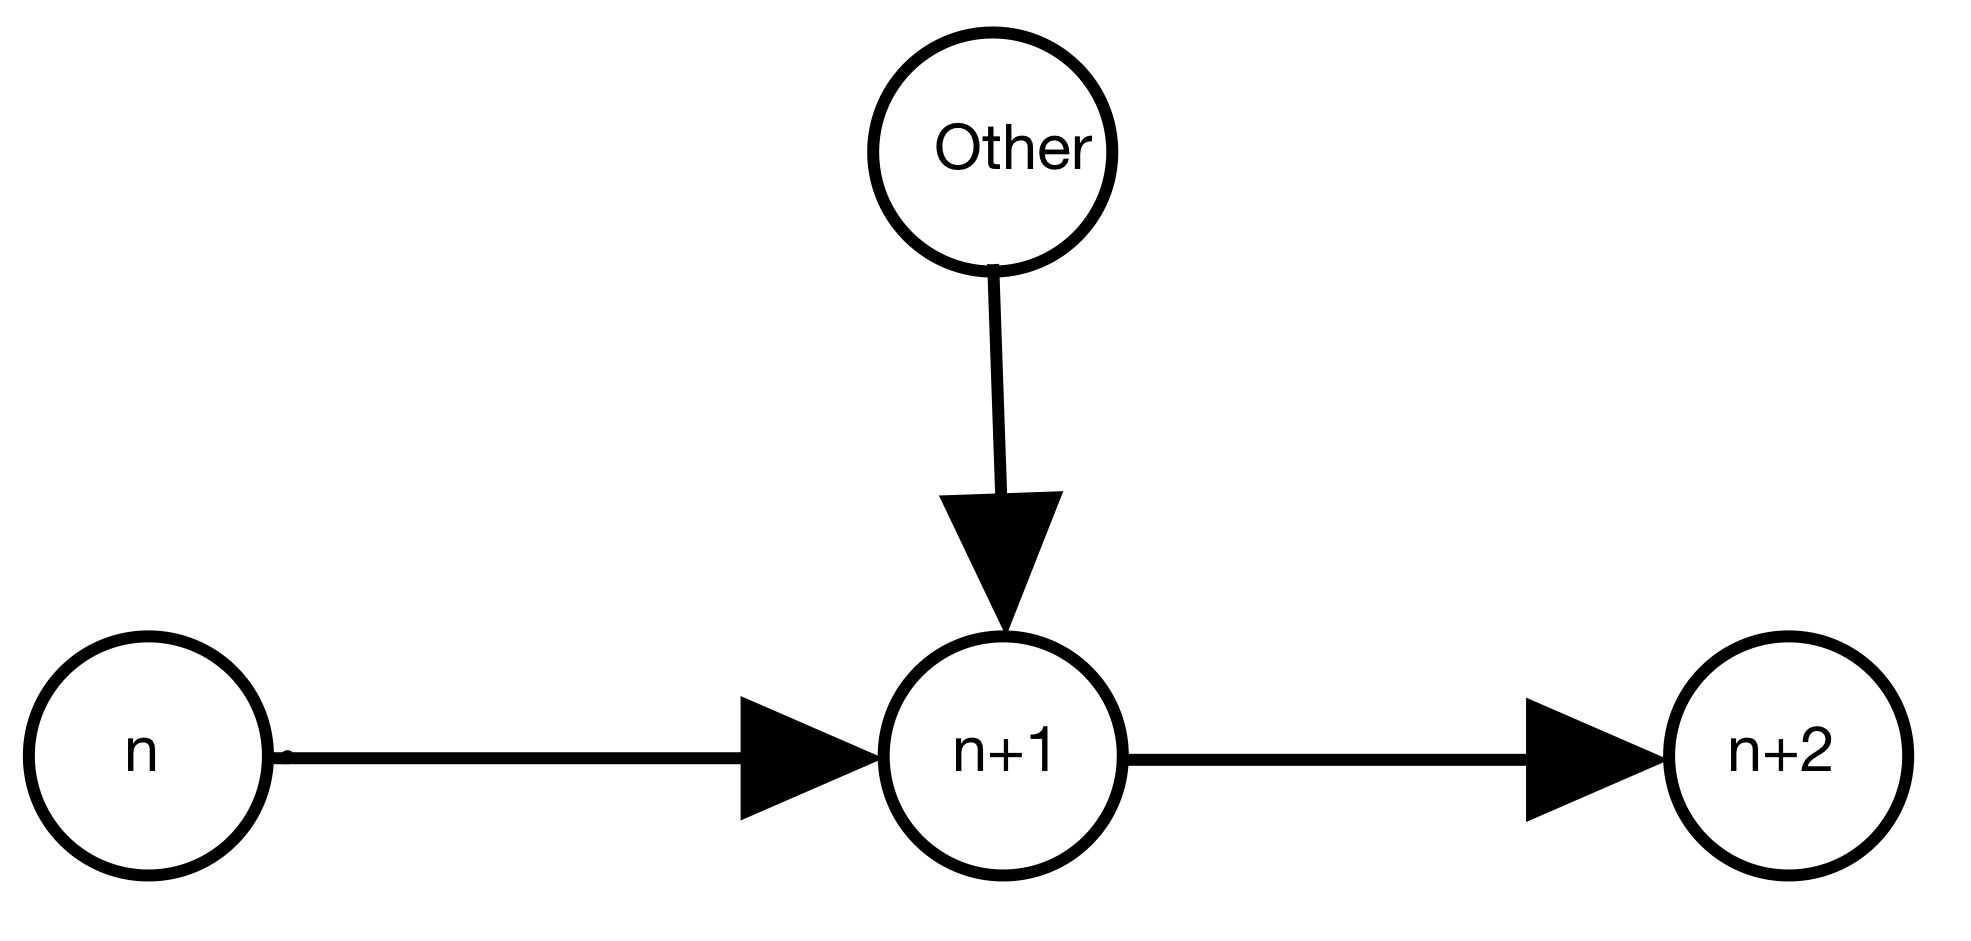
\includegraphics[width=.5\textwidth]{maerkefu.png}
	\caption{Indirect influence transmission chains}
	\label{img}
\end{figure}

In this process, we first assume that the node to which the follower belongs is inactive, and the influence of node n on node n+1 is $\eta_{nn+1} $, then the indirect influence of node n+1 on the node of the n+2 generation belonging to the first generation is:
\begin{equation}
q_{nn+2}=\frac{p _{nn+1}q_{nn+1}}{\Sigma p _{n+1}}\mathcal{P}  
\end{equation}
Where $\Sigma p _{n+1}$ represents the sum of the direct influence of all other nodes on node n+1, and $\mathcal{P}$ represents the attenuation degree of the indirect influence of node n on node n+2.

Obviously, $0\leqslant \mathcal{P} \leqslant 1$, So in this network, starting from node n, any node that can be reached through a directed segment will be indirectly influenced by node n so the indirect influence of node n should be the sum of these values, which is obviously of the form $\Sigma \alpha _{n}\mathcal{P} ^{n}$. So even though the whole network is huge, this value should converge. However, in order to prevent some artists from making this value too large to be reasonable due to the large number of indirect influences, we set a threshold $\mathbf{Q} $. When the indirect influence on a certain transmission chain is less than this threshold $\mathbf{Q} $, the transmission ends.

Here we set $\mathcal{P} $ as $0.5$, and we will test the sensitivity at the end of the paper.
So we get a quantitative measure of the total amount of influence that a node generates:
\begin{equation}
Inf_{i}=\Sigma p_{i}+\Sigma q_{i}
\end{equation}
Where $\Sigma p_{i}$ represents the sum of the quantized values of the direct influence of all nodes directly pointed to by node i, and $\Sigma q_{i}$ represents the sum of the quantized values of the indirect influence of all nodes having an indirect influence relationship with node i.

At the same time, through the reference of music history. We find that in the study of music history, people regard the connection between the three generations as a kind of inheritance. So we make $Q$ a little less than the indirect influence of the third generation artists. This can greatly simplify the calculation of the program.

\subsection{Some analysis of subnetworks}

We take the internal network of easy listening as the initial network, select all the artists associated with it from the whole complex network and join it to form a sub network.


\begin{figure}[H]
	\centering
	\begin{minipage}[t]{0.48\textwidth}
		\centering
		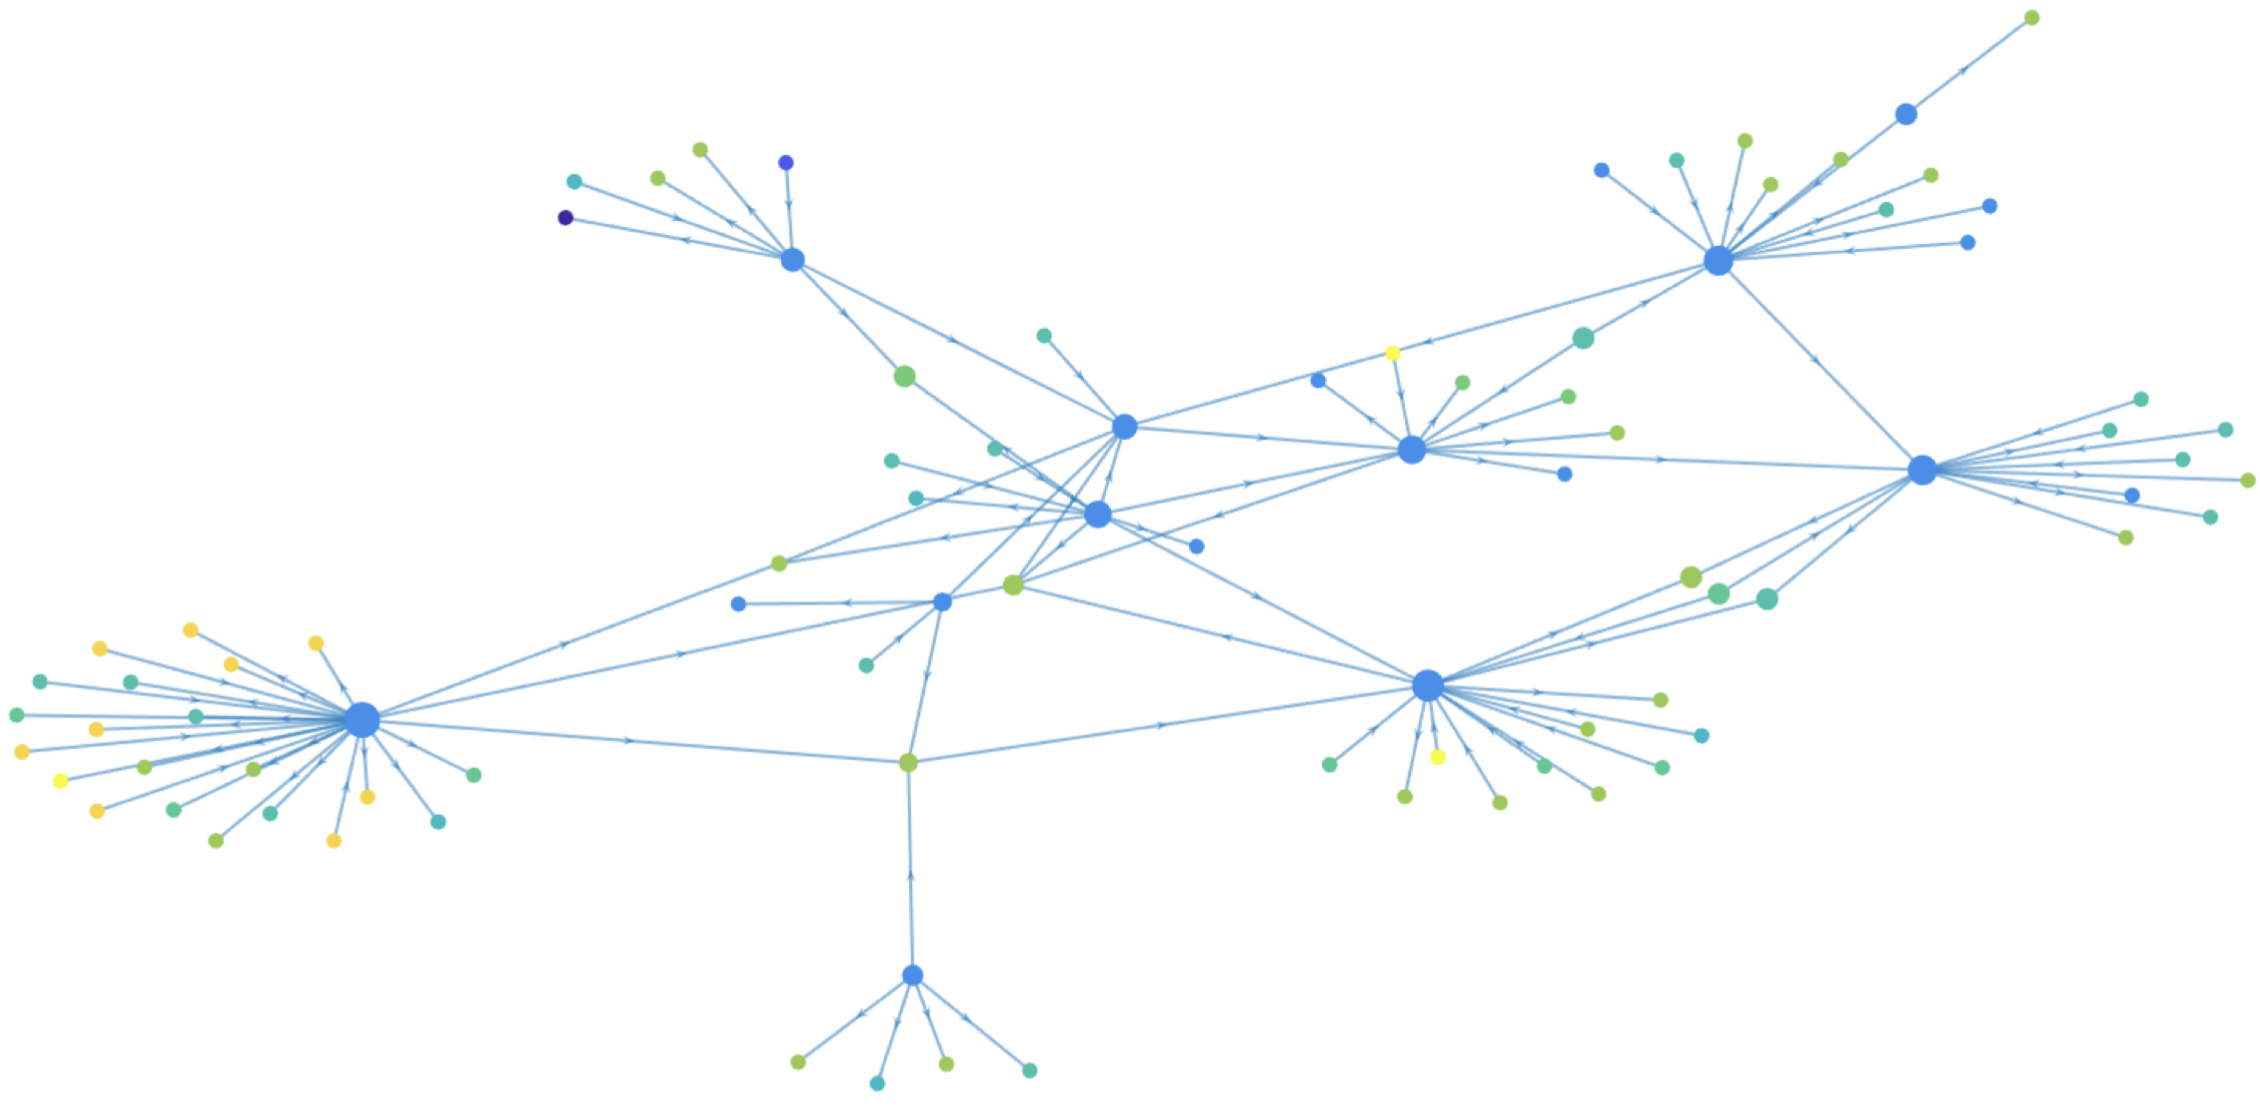
\includegraphics[width=8cm]{easyliten1.png}
		\caption{the subnetworks (different genres with different colors)}
	\end{minipage}
	\begin{minipage}[t]{0.48\textwidth}
		\centering
		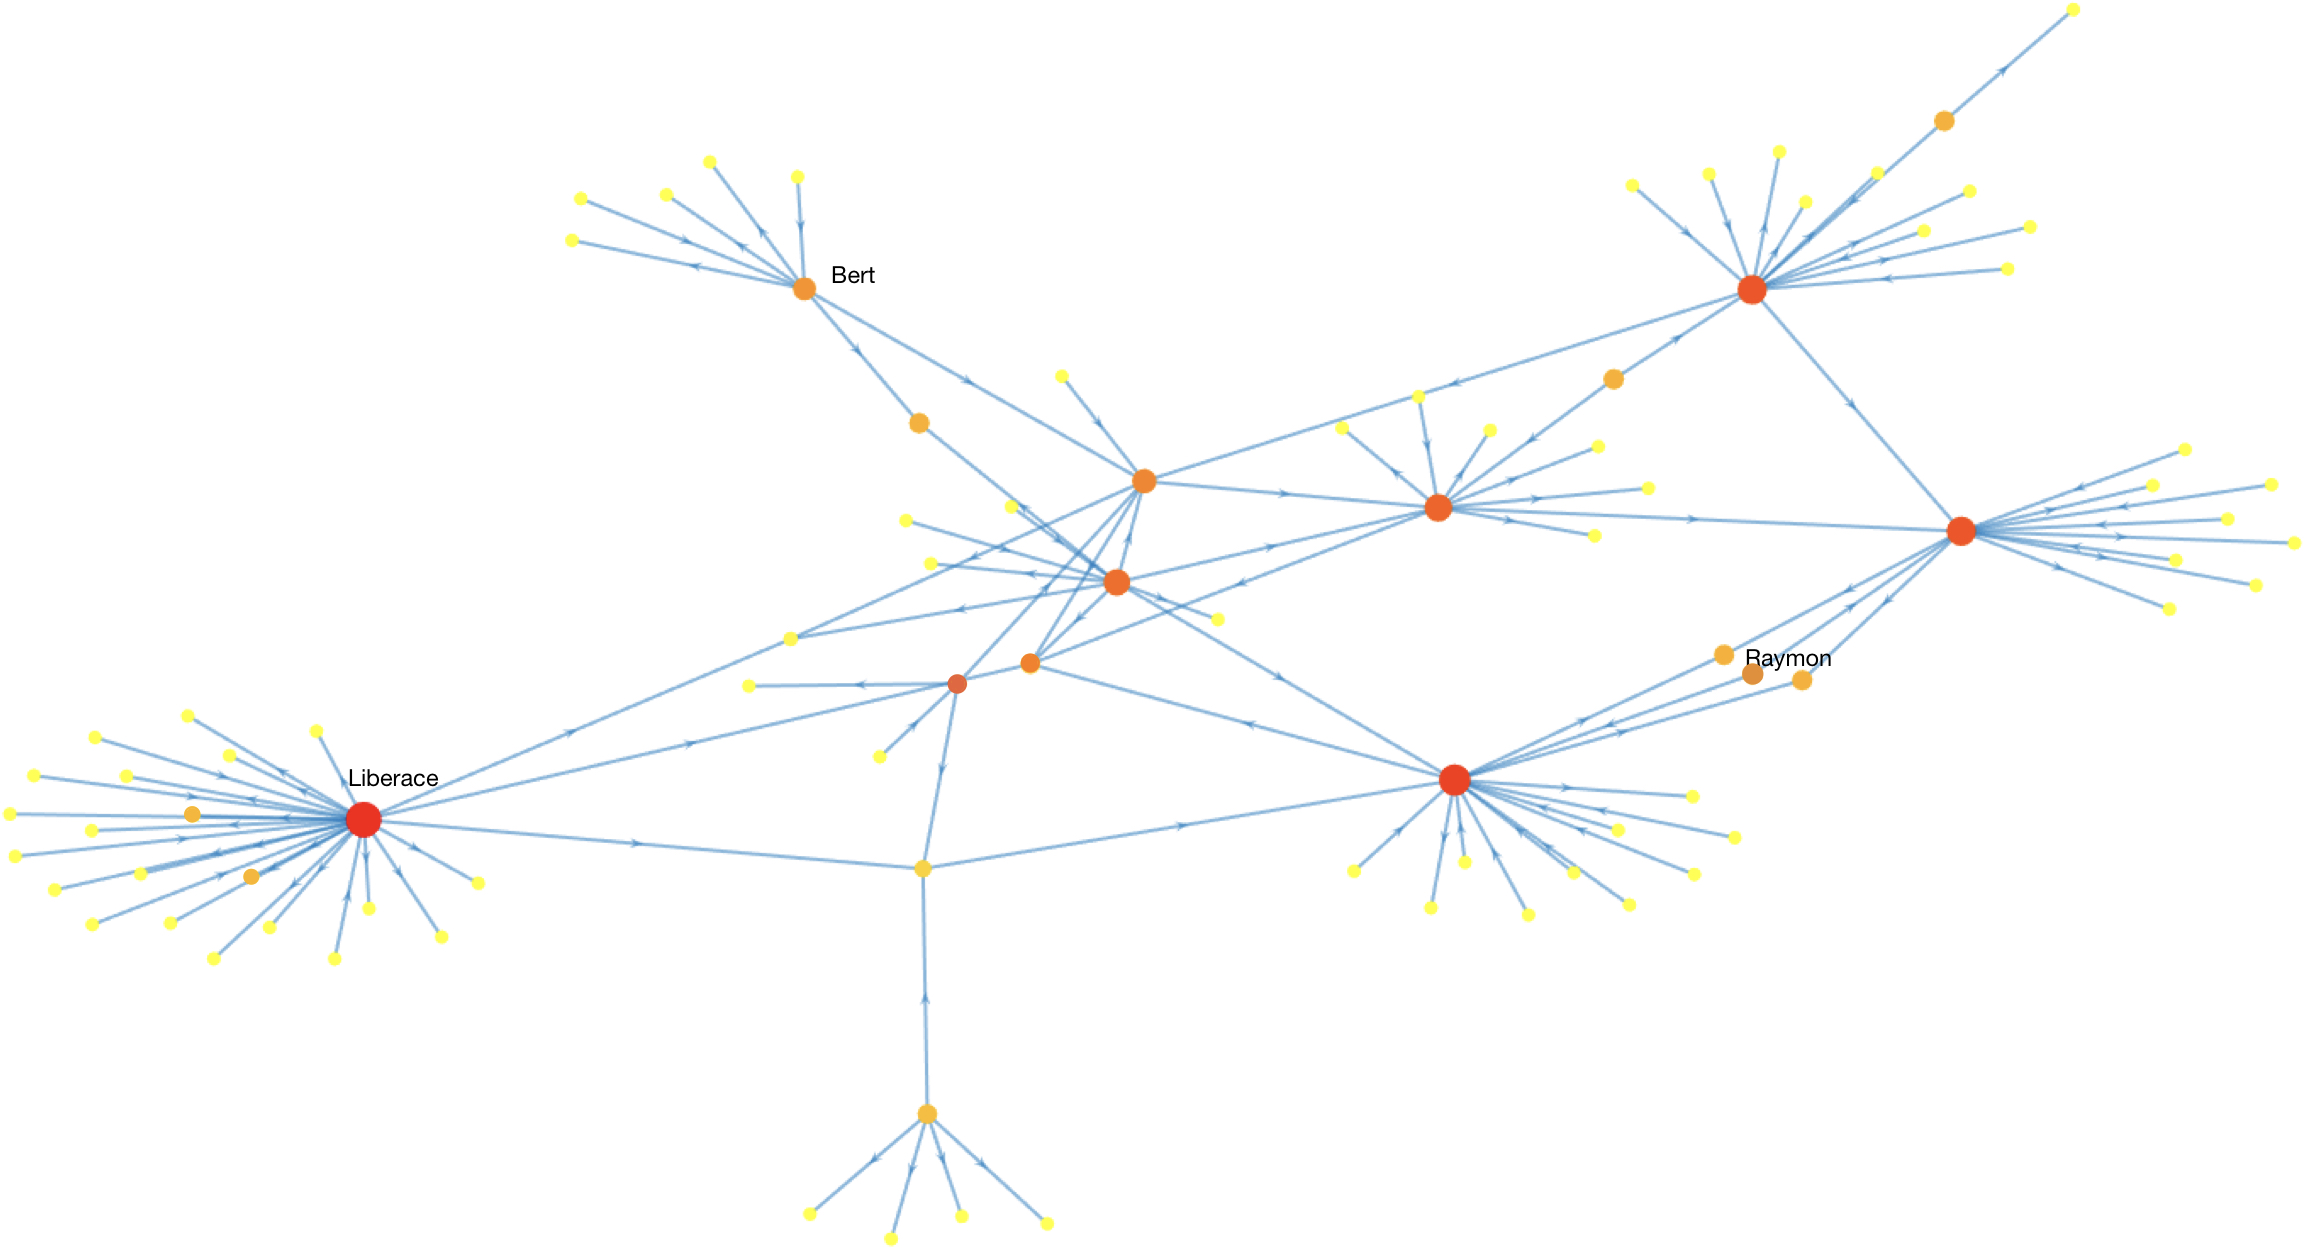
\includegraphics[width=8cm]{easylisten2.png}
		\caption{color depth with influence}
	\end{minipage}
\end{figure}

Through the comparison of the two pictures, we can clearly see that the artists who have a great influence in this sub network are the founders of this genre and some influential figures in this genre. By looking up the history of music, we find that Andr and Liberace, which correspond to these points, have a relatively important influence in this genre. At the same time, we found that some artists outside the genre, such as Raymond, also had a greater impact, because in the whole network, they had enough influence to influence other genres. This also verifies that the influence index inf established by us can well reflect the specific influence of an artist.


\section{Task2: Similarity model and Clustering}
\subsection{Similarity model}
\subsubsection{Preparation of the model}

For the quantification model of music similarity, we first extract the eigenvalues from the data set. Fortunately, the data set has classified the features of the song for us, and quantified each feature. But there are a lot of these features.

Therefore, we need to reduce the dimensionality of the data before building the similarity model.

We use the random forest algorithm to reduce its dimensionality,First we define the information entropy:
\begin{equation}
H(X)=-\sum_{i=1}^{n} m_{i} \log \left(m_{i}\right)
\end{equation}
where $m_{i}$  is the probability of occurrence of the event. After that we define the conditional entropy:
\begin{equation}
H(Y \mid X)=H(X, Y)-H(X)
\end{equation}
The information gain:
\begin{equation}
g(D, A)=H(D)-H(D \mid A)=I(D, A)
\end{equation}
The decision tree uses the Bootstrap Aggregating method to obtain the information gain of the features, and if the information gain is greater, the feature importance is greater.

We calculated all the eigenvalues and obtained their importance:

\begin{figure}[H]
    \centering
    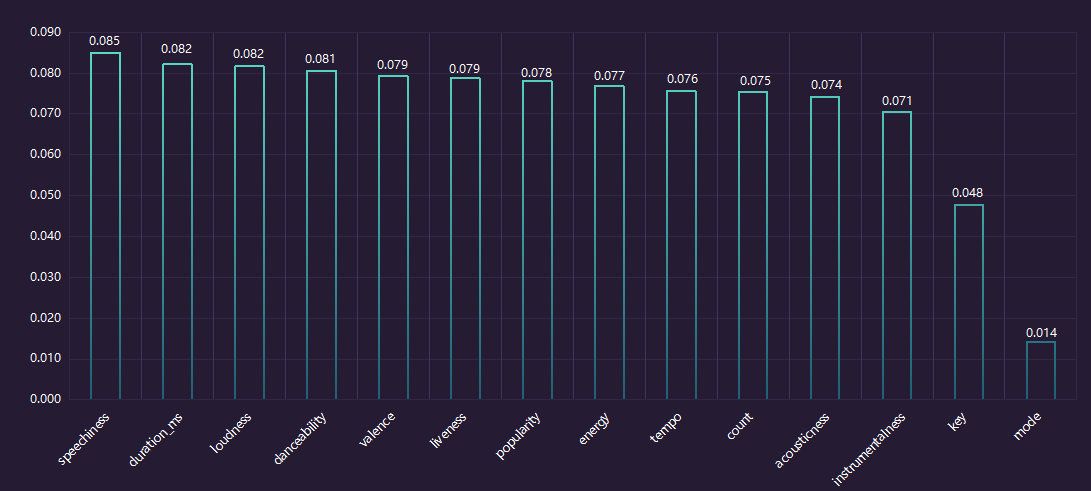
\includegraphics[width=.7\textwidth]{importancefeature.png}
    \caption{feature importance}
    \label{img}
\end{figure}
We set the valve field to 0.5, and we can see that the two quantities, Key and Mode, are obviously smaller than other quantities and are smaller than the valve field, so we eliminate these two eigenvalues.

\subsubsection{Establishment of the model}
Next, we take a set of eigenvalues of an artist as a vector:
\begin{equation}
\overrightarrow{X_i } =( x_{i1},x_{i2},\dots,x_{i12})
\end{equation}

They correspond to a, b, c, d of the artist $i$.

Then, for the similarity between any two artists, we can express it by the cosine of the Angle between two vectors.
\begin{equation}
C_{ij}=\frac{\overrightarrow{X_i}\cdot \overrightarrow{X_j}  }{\sqrt{\sum_{n = 1}^{12}x_{in}^2\cdot \sum_{n = 1}^{12}x_{jn}^2  } } 
\end{equation}
Obviously, the closer the absolute value of $c_{ij}$ is to 1, the higher the correlation. For the similarity, when $C_{ij}$ is low, it means that they are quite different.

Now, of course, up until this point, because each of these data classes have different dimensions, we normalized the data and we used what is called min-max Normalization. The transformation formula is as follows:
\begin{equation}
x^{*}=\frac{x-min}{max-min}
\end{equation}

To understand the relationship between artists and genres, we randomly selected ten artists from different genres, calculated their similarity to each other, and produced the following heat map:

\begin{figure}[H]
    \centering
    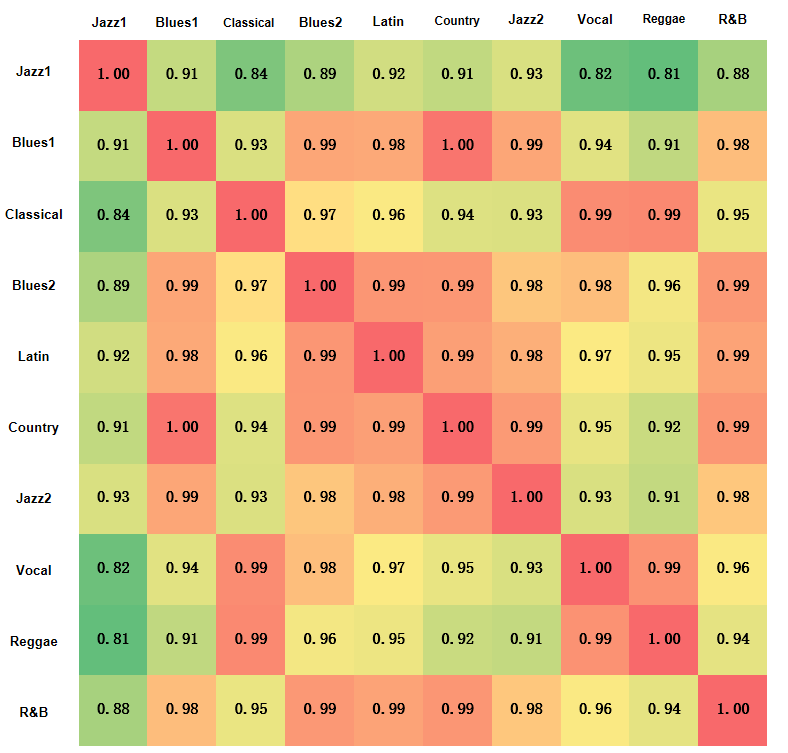
\includegraphics[width=.5\textwidth]{similarity.png}
    \caption{similarity}
    \label{img}
\end{figure}
\subsection{Hierarchical Clustering}
Then we conduct hierarchical clustering of these artists according to their similarity, so that we can get a classification map of them. By comparing this classification with their genre, we can know whether the similarity between artists is related to their genre.

Hierarchical clustering is a common way to categorize the data, here we stated briefly about this method First of all, we use the reciprocal of the similarity between artists to represent the distance $d_{ij}$ between $i$ and $j$:
\begin{equation}
d_{ij}=\frac{1}{c_{ij}}
\end{equation}
But for those nodes with negative similarity, we assume that the distance between them is greater than the distance between any set of nodes with positive similarity. Therefore, we define the distance between them as:
\begin{equation}
d_{ij}=1+\frac{1}{c_{ij}}
\end{equation}
And then all of the minimum distance $d_{pq}$ consolidation of the artists who are $p$ and $q$ involved into a class $r$, and that he and other artists is defined as the distance between them both average distance with other artists.

That is:
\begin{equation}
d_{rs}=\frac{1}{2}(d_{ps}+d_{qs})
\end{equation}
And so on until everyone is in the same category. 


The result is shown in the figure:

\begin{figure}[H]
    \centering
    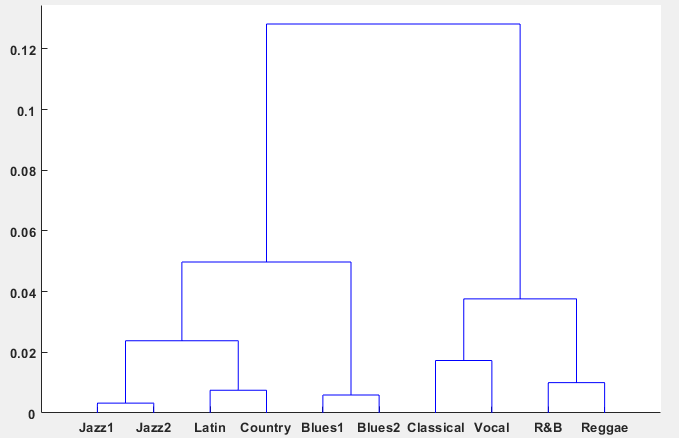
\includegraphics[width=.4\textwidth]{Hierarchical clustering result.png}
    \caption{Hierarchical clustering result}
    \label{img}
\end{figure}

We can see that in the same genre blues1 and blues2, jazz1 and jazz2 indeed have a higher similarity, that is to say, the artist has a higher similarity of the same genre But some artists may be in a border of two schools, the birth of at the same time they also bring some changes to the genre and development.

\section{Task3: Similarities and influences}
\subsection{Similarities and influences within the genre}
In order to compare the degree of similarity and influence within genres, we need to compare the similarity of the styles of some artists within a specific genre.

We have selected some of the artists in the Easy Listening genre as examples for our analysis, and their influence relationships are shown in the figure below:

\begin{figure}[H]
	\centering
	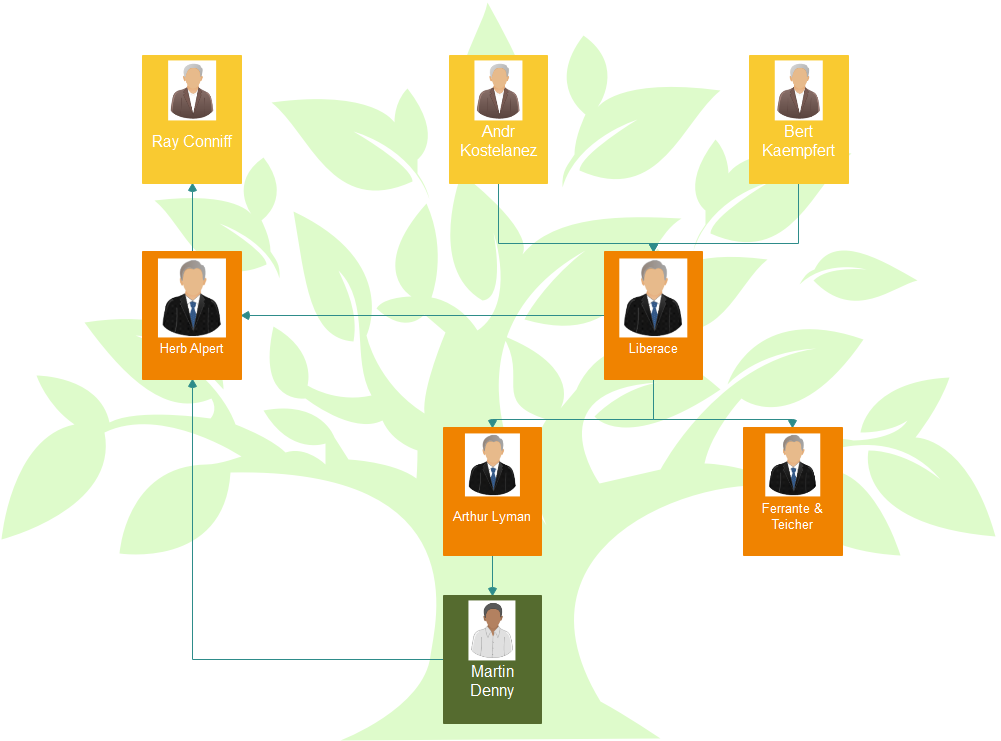
\includegraphics[width=.7\textwidth]{t31.png} 	% 图片相对位置
	\caption{Selected artist-influenced relationships in the Easy Listening genre}		% 图片标题 
	\label{fig:ex4-9}
\end{figure}

We first examine the three artists Liberace, Arthur Lyman, and Ferrante \& Teicher, according to the figure above, Liberace influenced Arthur Lyman and Ferrante \& Teicher, and we select the average of all three of their works based on their influence. The results are shown below. The results are shown in the following figure:

\begin{figure}[H]
	\centering    
	\subfigure[Comparison of the styles of Liberace, Arthur Lyman, Ferrante \& Teicher's works]{				% 图片1([]内为子图标题)
		\label{fig:sub.roomhot}							% 子图1的标签
		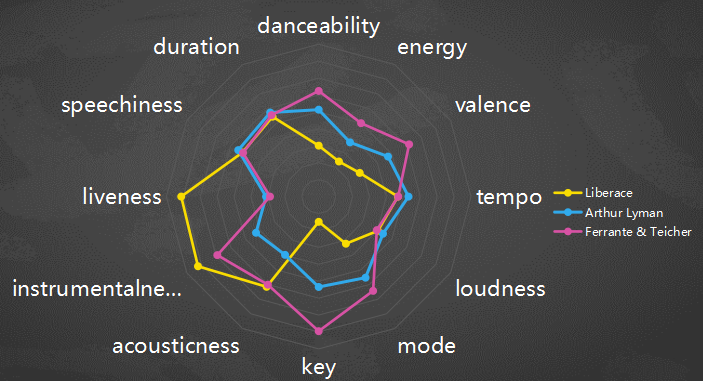
\includegraphics[width=0.5\textwidth]{t32.png}}% 子图1的相对位置
	\subfigure[Comparison of the styles of Arthur Lyman and Martin Denny's works]{				% 图片2
		\label{fig:sub.floorhot}						% 子图2的标签
		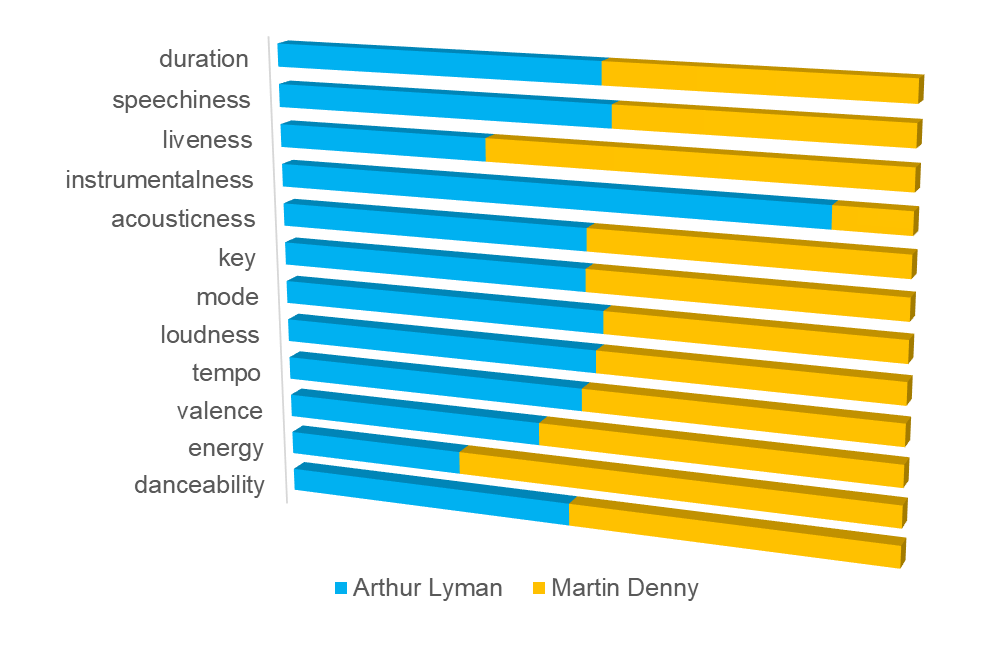
\includegraphics[width=0.45\textwidth]{t33.png}}% 子图2的相对位置
	\caption{Comparison of artisits}		% 总图标题
	\label{fig:hot}									% 总图标签
\end{figure}


From the figure, we can see that the three artists remain highly similar in duration, speechiness, tempo, and loudness, verifying that Arthur Lyman and Ferrante \& Teicher are influenced by Easy Listening in several distinctive aspects. Liberace, but the differences in liveness are significant, suggesting that as the network evolves, the later members of the genre perform less live. Moreover, danceability, energy, and validity have all improved compared to Liberace in the 1940s, suggesting that the music of Easy Listening was gradually developed to be more danceable, energetic, and active.

After that, we then analyzed the characteristics of the works of Arthur Lyman and the follower Martin Denny, and the results are shown in Figure 10(b)

From the diagram, we can find that the characteristics of Arthur Lyman and Martin Denny's works are mostly similar, except for the three characteristics of energy, liveness, and instrumentalness, which may be influenced by the environment. This shows that Arthur Lyman has a great influence on the style of Martin Denny's works.

\subsection{Similarities, differences and influences between genres}
In order to explore the similarities, differences and influences between genres, we expressed the characteristic quantity of each genre in terms of the average characteristic quantity of all works in that genre based on the data in the full\_music\_data and influence\_data tables. And we visualize it as shown in the figure below:

\begin{figure}[H]
	\centering
	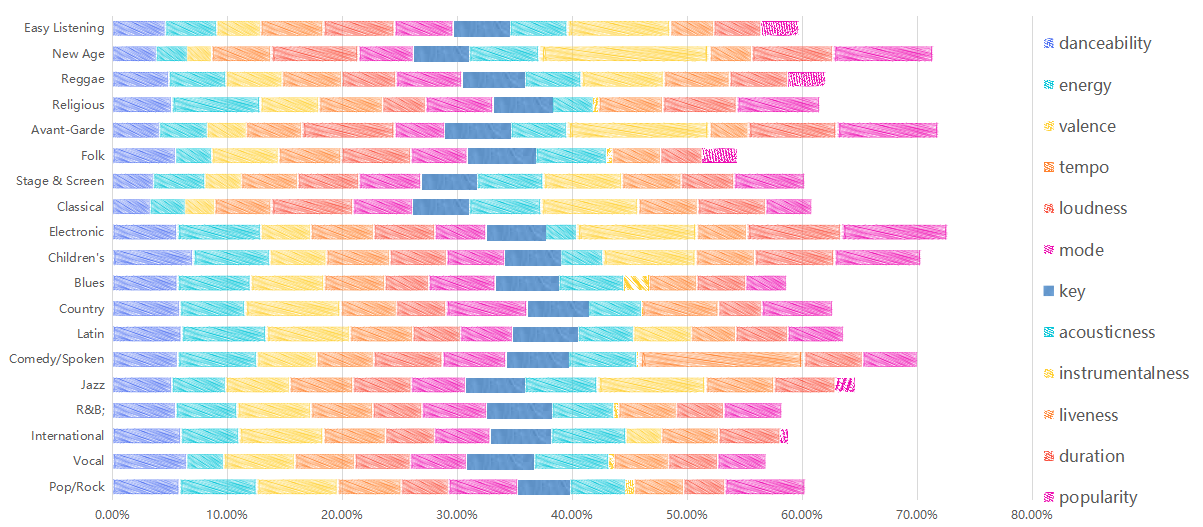
\includegraphics[width=.8\textwidth]{t34.png} 	% 图片相对位置
	\caption{Comparison of the styles of each genre}		% 图片标题 
	\label{fig:ex4-9}
\end{figure}

\subsection{Changes in genre over time}
In order to explore the changes that occur in a genre over time, we analyze the classical genre as an example.

We counted the mean values of each attribute at each interval from 1930-2010, after which we calculated its standard deviation, where the four attributes of valence, instrumentalness, popularity, and key fluctuate significantly, and we made a graph of them as follows:
\begin{figure}[H]
	\centering
	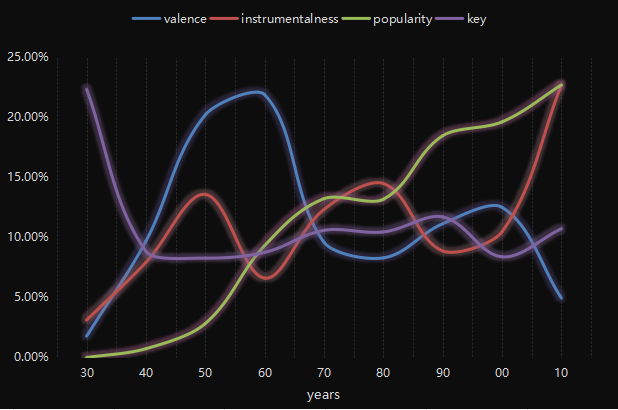
\includegraphics[width=.5\textwidth]{t36.png} 	% 图片相对位置
	\caption{Changes in classical genres over time}		% 图片标题 
	\label{fig:ex4-9}
\end{figure}
We can see a general upward trend in the popularity of classical music, with the 1940s being the turning point for key, compared to the 1930s, when the tone of classical music slowed down from the 1940s and was inherited all the way through. at the same time, valence increased sharply in the 1940s, which we presume was influenced by the Second World War. 

The 1950s were the turning point for instrumentalness turned a corner, with a sharp decrease in instrumentalness values, accompanied by a further increase in valence values to a peak, indicating the inclusion of more vocals in the music and a high level of emotion. In the 60s, the values of valence decreased sharply, accompanied by an increase in instrumentalness, indicating that the effect of certain events that occurred in the 50s In the 1970s, the popularity of classical music declined for the first time, while other characteristics changed little, probably due to the influence of the explosion of other musical styles. 

\subsection{The connection between genres}
In order to explore the degree of association between genres, we first analyze them from the perspective of the originator. We define the originator of a genre as the artist who first developed the style and influenced the largest number of people within the genre.

We counted the originators of all genres and the relationships of influence between them, as shown in the following figure:

\begin{figure}[H]
	\centering
	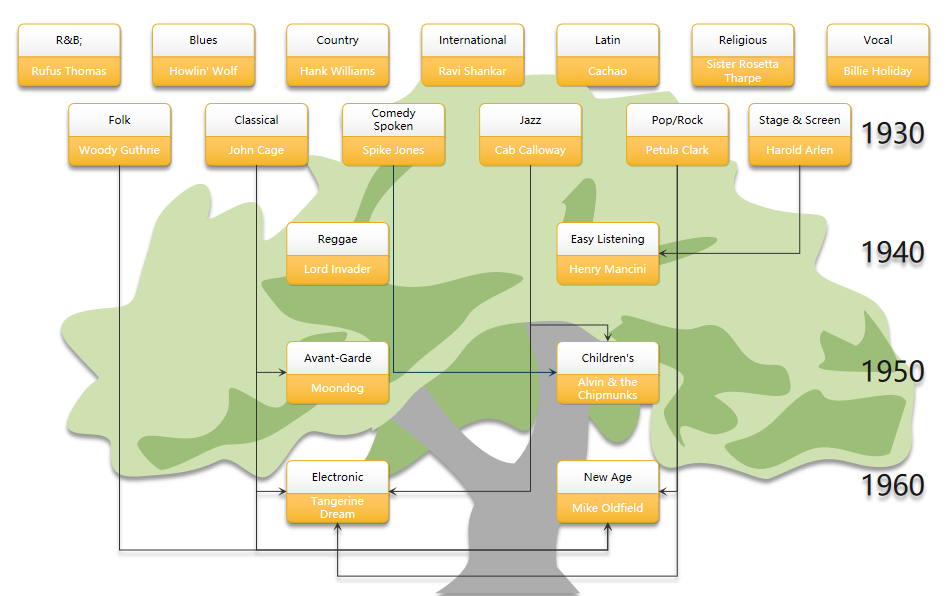
\includegraphics[width=.7\textwidth]{t37.png} 	% 图片相对位置
	\caption{The relationship of influence between the originators of each school}		% 图片标题 
	\label{fig:ex4-9}
\end{figure}

In the figure, we find 15 genres whose originators were formed in the 1830s, and in the 1840s, the Reggae and Easy Listening genres emerged, where Henry Mancini, the originator of Easy Listening, was influenced by Haroid Arlen, the originator of Stage\&Screen. Arlen's influence led to the creation of Easy Listening.

In the same way that the Avant-Garde genre was influenced by the Classical genre in the mid-1850s, the Children's genre was influenced by the Jazz genre and the Comedy Spoken genre together. By the 1860s, the Electronic genre emerged from the combined influence of the Jazz and Classical genres and the Pop/Rock genre, and the New Age genre was born from the combined influence of the Classical and Pop/Rock genres.

Based on the data of works in each genre, we can dig out the salient features of each genre, as shown in the following table:

\begin{table}[H]
	\centering
	\begin{tabular}{|c|c|c|}
		\hline
		Genre           & \multicolumn{2}{c|}{Characteristic} \\ \hline
		Pop/Rock        & energy           & valence          \\ \hline
		Vocal           & danceability     & acousticness     \\ \hline
		International   & valence          & acousticness     \\ \hline
		R\&B            & valence          & key              \\ \hline
		Jazz            & acousticness     & instrumentalness \\ \hline
		Comedy/Spoken   & speechiness      & explicit         \\ \hline
		Latin           & energy           & valence          \\ \hline
		Country         & valence          & mode             \\ \hline
		Blues           & energy           & valence          \\ \hline
		Children's      & danceability     & instrumentalness \\ \hline
		Electronic      & instrumentalness & duration         \\ \hline
		Classical       & instrumentalness & explicit         \\ \hline
		Stage \& Screen & acousticness     & instrumentalness \\ \hline
		Folk            & key              & acousticness     \\ \hline
		Avant-Garde     & loudness         & instrumentalness \\ \hline
		Religious       & energy           & tempo            \\ \hline
		Reggae          & mode             & instrumentalness \\ \hline
		New Age         & instrumentalness & duration         \\ \hline
		Easy Listening  & loudness         & instrumentalness \\ \hline
	\end{tabular}
	\caption{Characteristics of each genre}
\end{table}

From the table we can get the same characteristics of these genres, such as Pop/Rock, International, R\&B, Latin, Country, and Blues all have significant values of valence, which means that their music is full of positive emotions.

\section{Task4 :The relationship between influencers and followers}

\subsection{The relationship between the works of influencers and followers}

To explore whether followers' musical styles are influenced by influencers, we need to consider the following online scenario, where one artist follows multiple influencers at the same time. 

Taking Al Di Meola in The 1970s as an example, according to The data of influence-data, he was influenced by six artists including Julian Bream, John McLaughlin, Jim Hall, Jimi Hendrix, Miles Davis, and The Beatles. The network structure is shown as follows:

\begin{figure}[H]
    \centering
    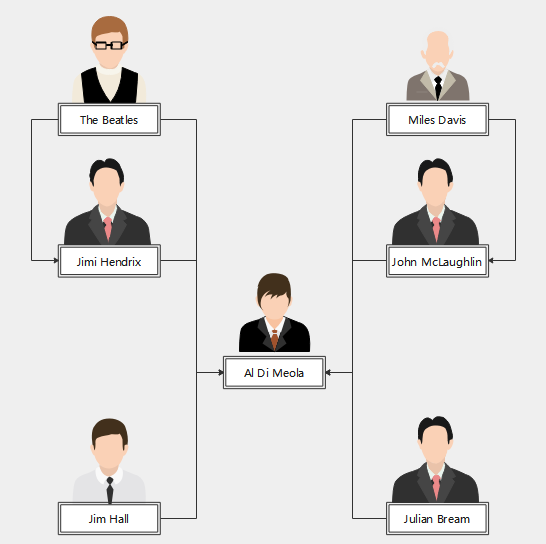
\includegraphics[width=.4\textwidth]{AL Di.png}
    \caption{Network structure of Al Di Meola}
    \label{img}
\end{figure}

We use the statistical data in data\_artists table to formulate corresponding eigenvalue phasor for each of their works, and then calculate the similarity between artists as followers and influencers.

Meanwhile, according to the influence model in Task1, we calculate the influence of six influenders, among which John McLaughlin, Jim Hall, Miles Davis and followers Al Di Meola belong to the same Jazz genre, while the others belong to different genres.

The results are as follows:

\begin{table}[H]
    \centering
    \begin{tabular}{lcc}
    \hline
    \hline
                                          & \textbf{influence} & \textbf{simarity}           \\ \hline
    \textbf{The Beatles}                  & 0.7864             & 0.8429                      \\
    \textbf{John McLaughlin}              & 0.6794             & 0.7627                      \\
    \textbf{Miles Davis}                  & 0.4376            & -0.3557 \\
    \textbf{Jimi Hendrix}                 & 0.3467            & 0.2738                      \\
    \textbf{Jim Hall}                     & 0.2467             & -0.1849 \\
    \textbf{Julian Bream}                 & 0.1349            & 0.0705                      \\ \hline
    \hline
    \end{tabular}
    \caption{the table of influence and simarity}
\end{table}
It can be found from the table that Miles Davis and Jim Hall had a negative influence on Al Di Meola, indicating that Al Di Meola innovated the style of Miles Davis and Jim Hall's works, while he basically inherited the style of others' works. 

If we only consider the numerical size, we find that the influence of the influencer is related to the similarity between the influencer and the follower's works, that is, the more influential the person is, the more likely the follower will imitate him. But at the same time, some artists will be influenced by some influential artists and make some big changes to the style of the influencer to form their own style.

\subsection{Influence factor}

In order to further explore which features of influentials' works influenced their followers, we selected two of them, The Beatles and John McLaughlin, who had The greatest influence on The style of Al Di Meola's works, and analyzed The detailed data of all aspects of their works, as shown in The figure below

\begin{figure}[H]
    \centering
    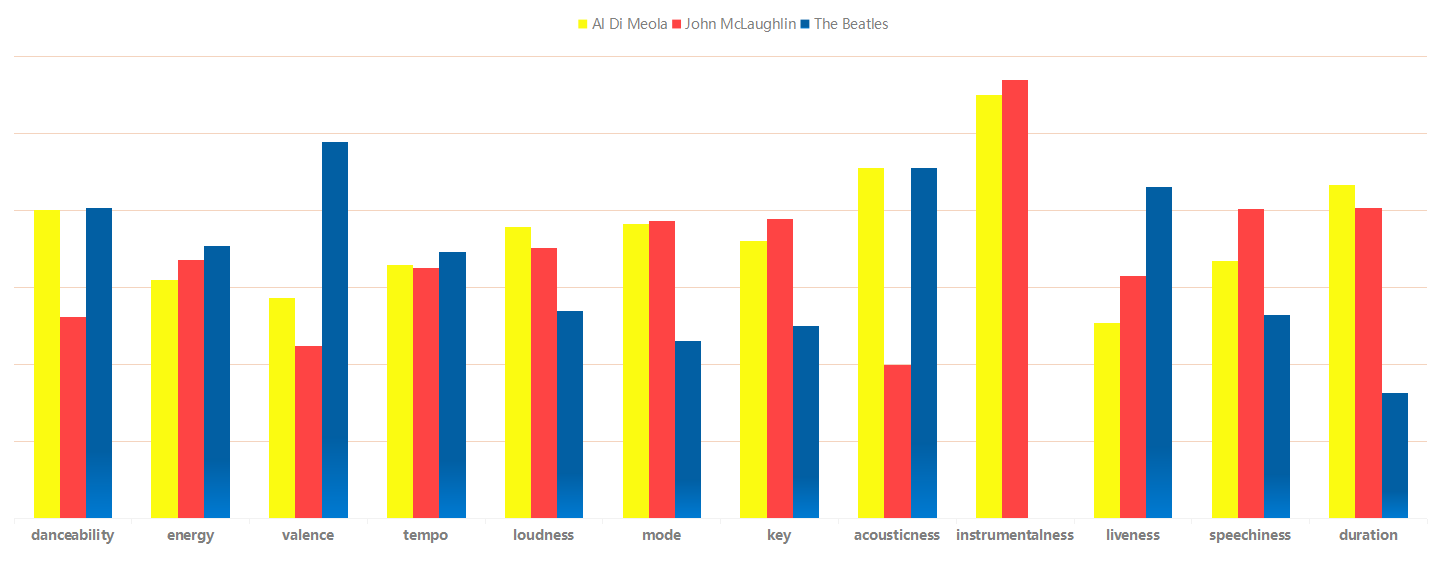
\includegraphics[width=.8\textwidth]{factors.png}
    \caption{eigenvalue comparison}
    \label{img}
\end{figure}

We can see from The table, The AI DI Meola in tempo, mode, key, instrumentalness, mainly inherited The style of The John Mclaughlin duration, in danceability acousticness aspects mainly inherited The style of The Beatles.

So we can conclude that influencers are contagious in certain ways.

\section{Task5: Features and Leaders for change}
\subsection{Features that produce change}
In order to identify revolutionary features in the evolution of music, we can take a decade as a time unit and plot the change curve of each feature of the genre over time, and if there is a large fluctuation, the feature belongs to a major leap.

We counted folk genre from the 1950 s to 2010 s work characteristics change, we calculate the variance of each characteristic value, after selecting the obvious fluctuations in the eigenvalue instrumentalness, speechiness and popularity made their variation, the result is shown in the following figure:

\begin{figure}[H]
    \centering
    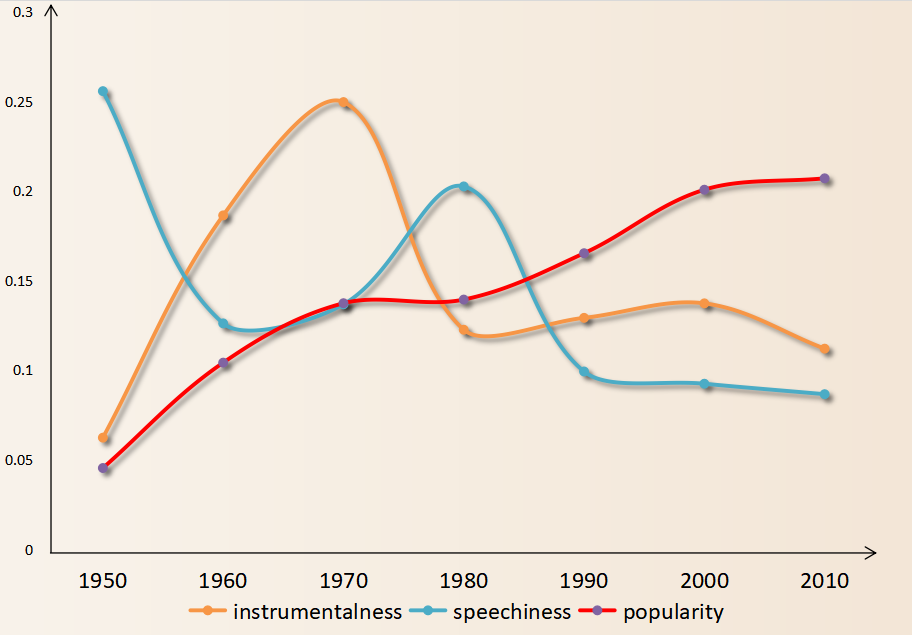
\includegraphics[width=.7\textwidth]{t61.png}
    \caption{Some change in eigenvalues}
    \label{img}
\end{figure}

From the graph we can see that in the 20 years from 1950 to 1970, there was a sharp decline in speechiness, accompanied by a sharp rise in instrumentalness, which, combined with a dramatic increase in popularity, leads us to speculate that perhaps folk emerged as the star artists who drove the genre forward.

\subsection{Explore leaders for change} 

To explore who caused this change, we extracted the characteristics of all artisits within the genre in that time period, and used the cosine similarity in task2 to calculate the degree of similarity between the characteristics of their artisits' works and the characteristics of the genre between this point in time. If the degree of similarity is greater and the artist has some influence, then he is the change agent of the genre.

We have listed some of the most influential artists in the 1950s and Folk genre. The results are shown below:

\begin{table}[H]
    \centering 
    \begin{tabular}{ccc}
    \hline
    \hline
    \multicolumn{1}{c|}{Name}                       & \multicolumn{1}{l}{simarity} & influence \\ \hline
    \multicolumn{1}{c|}{The Kingston Trio}     & 0.948                        & 8.96      \\
    \multicolumn{1}{c|}{Ramblin' Jack Elliott} & 0.903                        & 10.2      \\
    \multicolumn{1}{c|}{John Fahey}            & 0.877                        & 9.31      \\
    \multicolumn{1}{c|}{Joan Baez}             & 0.702                        & 15.5      \\
    \multicolumn{1}{c|}{Dave Van Ronk}         & 0.852                        & 9.74      \\ \hline
    \hline
    \end{tabular}
	\caption{Similarity and influence of some Folk genre artists}
\end{table}

From the table, we can find that Joan Baez is the artist who has the most influence and whose style is most inconsistent with the previous style of the genre. Therefore, we can infer that Joan Baez is a reformer of this era.

We select the average data of his works in this period and the average data of all Folk works in this period to calculate the distance between them, and measure his contribution to the style of the genre. The farther away from the average, the greater the contribution is. The result is shown in the figure below:

\begin{figure}[H]
    \centering
    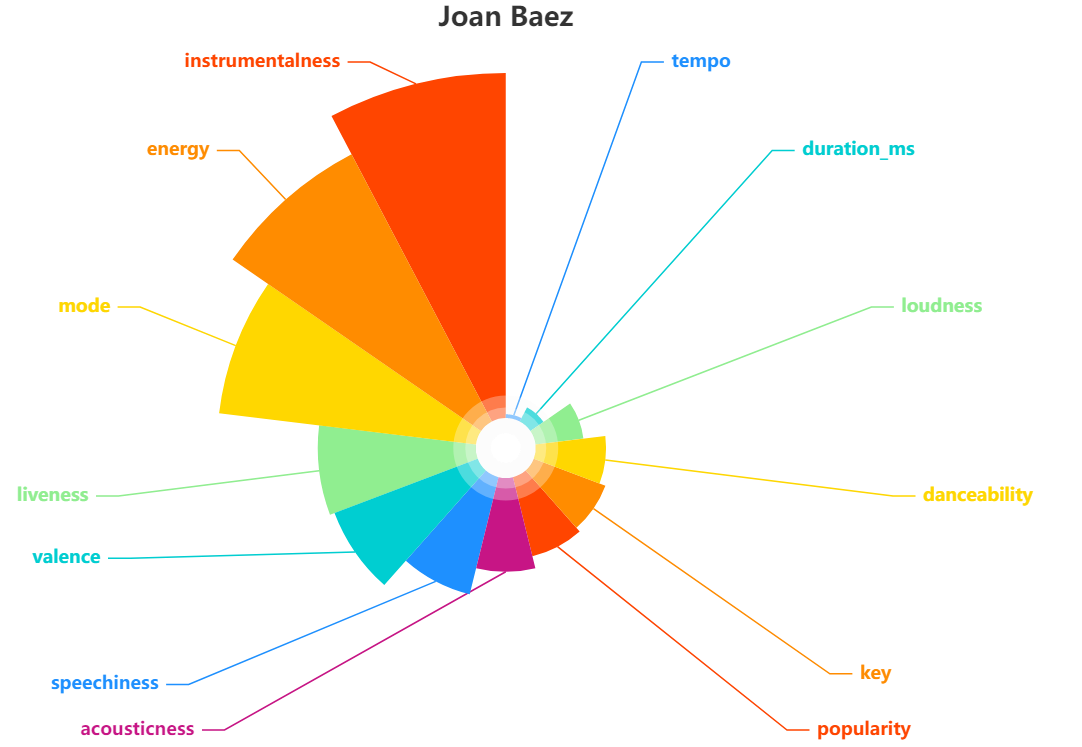
\includegraphics[width=.7\textwidth]{t62.png}
    \caption{Joan Baez}
    \label{img}
\end{figure}

From the graph, we can find that the contribution of Joan Baez's instrumentalness feature far exceeds the other features, so we can be sure that Joan Baez is the driving force that caused the stylistic change in the Folk genre.


The history of the development of the Folk genre\upcite{2}.
 shows that in the 1960s, Joan Baez combined the Folk genre with the Rock genre, introducing rock instruments such as the guitar to the Folk genre, thus driving a significant increase in the Folk genre's instrumentalness characteristics, further supporting our speculation.

We used the same method to filter out other genre changers and the results are shown in the following table:

\begin{table}[H]
	\centering
	\begin{tabular}{|l|l|l|l|l|}
		\hline
		Genre & Avant-Garde          & Blues           & Children's      & Classical      \\ \hline
		Name  & Terry Riley          & Muddy Waters    & Alvin           & John Cage      \\ \hline
		Genre & Latin                & New Age         & Pop/Rock        & R\&B;          \\ \hline
		Name  & Antnio Carlos Jobim  & Mike Oldfield   & The Beatles     & Marvin Gaye    \\ \hline
		Genre & Comedy/Spoken        & Country         & Easy Listening  & Electronic     \\ \hline
		Name  & Spike Jones          & Johnny Cash     & Henry Mancini   & Kraftwerk      \\ \hline
		Genre & Reggae               & Religious       & Stage \& Screen & Vocal          \\ \hline
		Name  & Toots \& the Maytals & James Cleveland & Ennio Morricone & Billie Holiday \\ \hline
		Genre & International        & Easy Listening  & Jazz            &                \\ \hline
		Name  & Ravi Shankar         & loudness        & Miles Davis     &                \\ \hline
	\end{tabular}
	\caption{Change makers in every genre}
	\label{tab:my-table}
\end{table}

\section{Task6: Genre evolution}
\subsection{Dynamic index of genre evolution}
According to the community model of Task1, we can regard a genre in the influence network as a community. When a genre changes greatly, the variance of the similarity of songs belonging to this genre in this period will expand. When the songs of this genre tend to be unified, their variance will decrease. We define the dynamic variance is "$\varphi $".

And then, we ues 10 years as a period to get a change chart of $\varphi (t)$:

\begin{figure}[H]
	\centering
	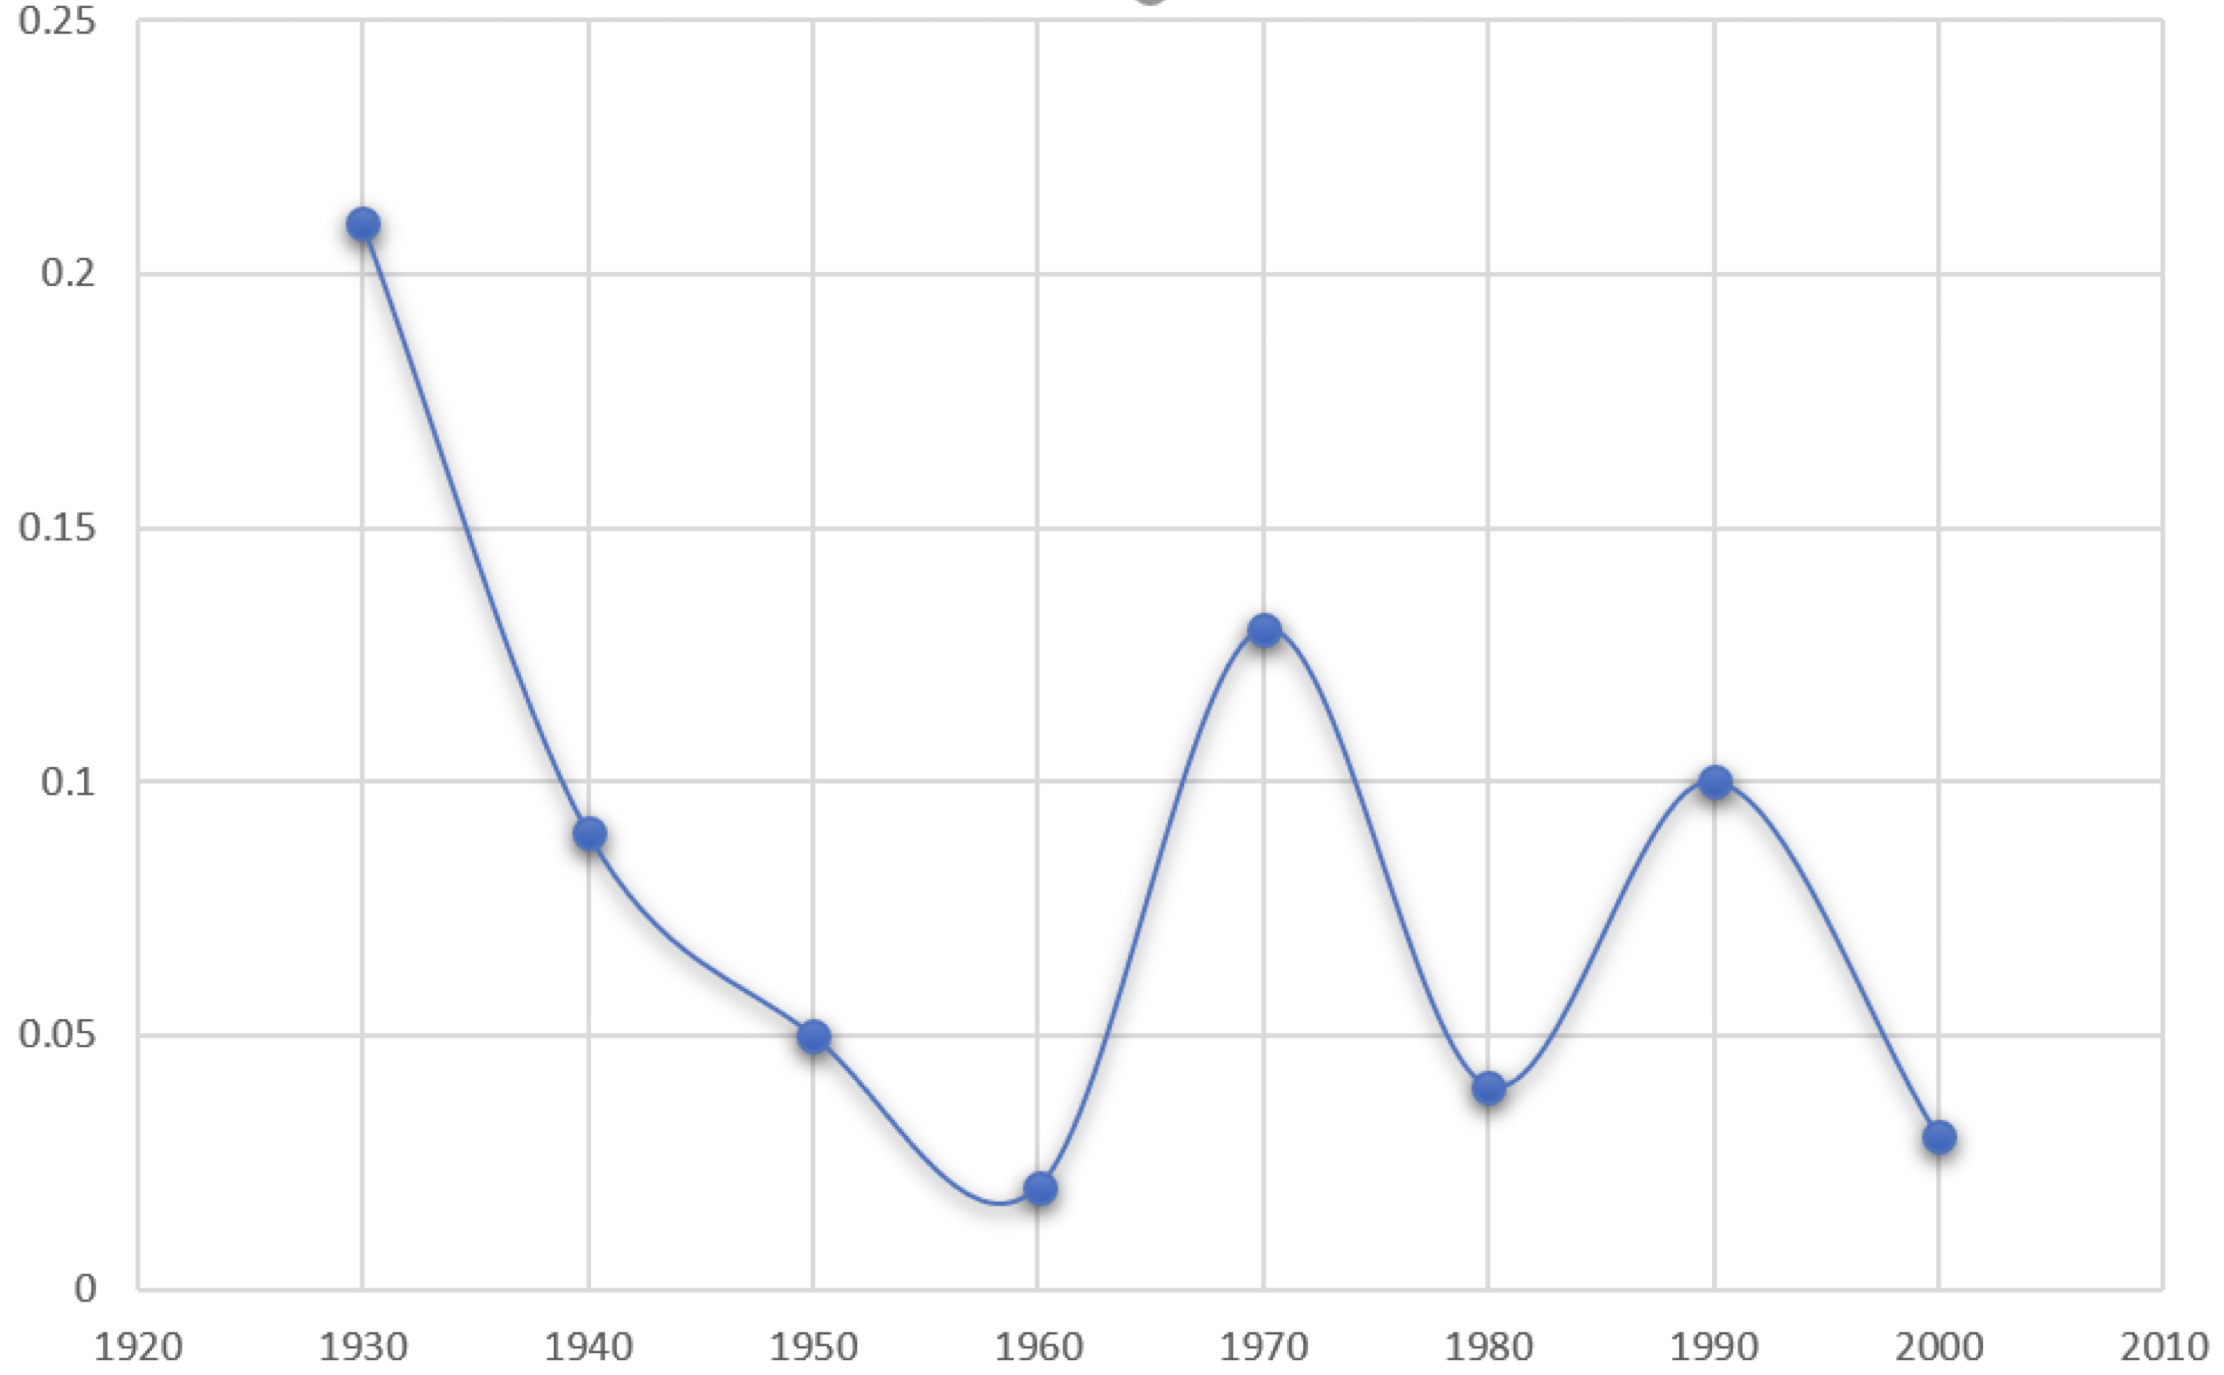
\includegraphics[width=.5\textwidth]{change.png}
	\caption{Variance of similarity over time}
	\label{img}
\end{figure}

We can intuitively see that the vocal school was in the era of change in 1930s and 1970s. At other times, the style area is stable.

But at the same time, the vitality of a school is also an important indicator to measure the change of a school. For a community in a network, we introduce the view of dynamic network to record the snapshot of network structure in each period. We use the size of the node to represent the degree of activity within the network, and use the links with other schools to represent the degree of communication activity with other schools. Finally, we use the sum $\psi $ of the size and degree of the node and  the node to represent the prosperity and decline of a community.
\begin{equation}
\psi (t)=size(t)+indegree(t)+outdegree(t)
\end{equation}
\begin{figure}[htbp]
	\centering
	\begin{minipage}[t]{0.48\textwidth}
		\centering
		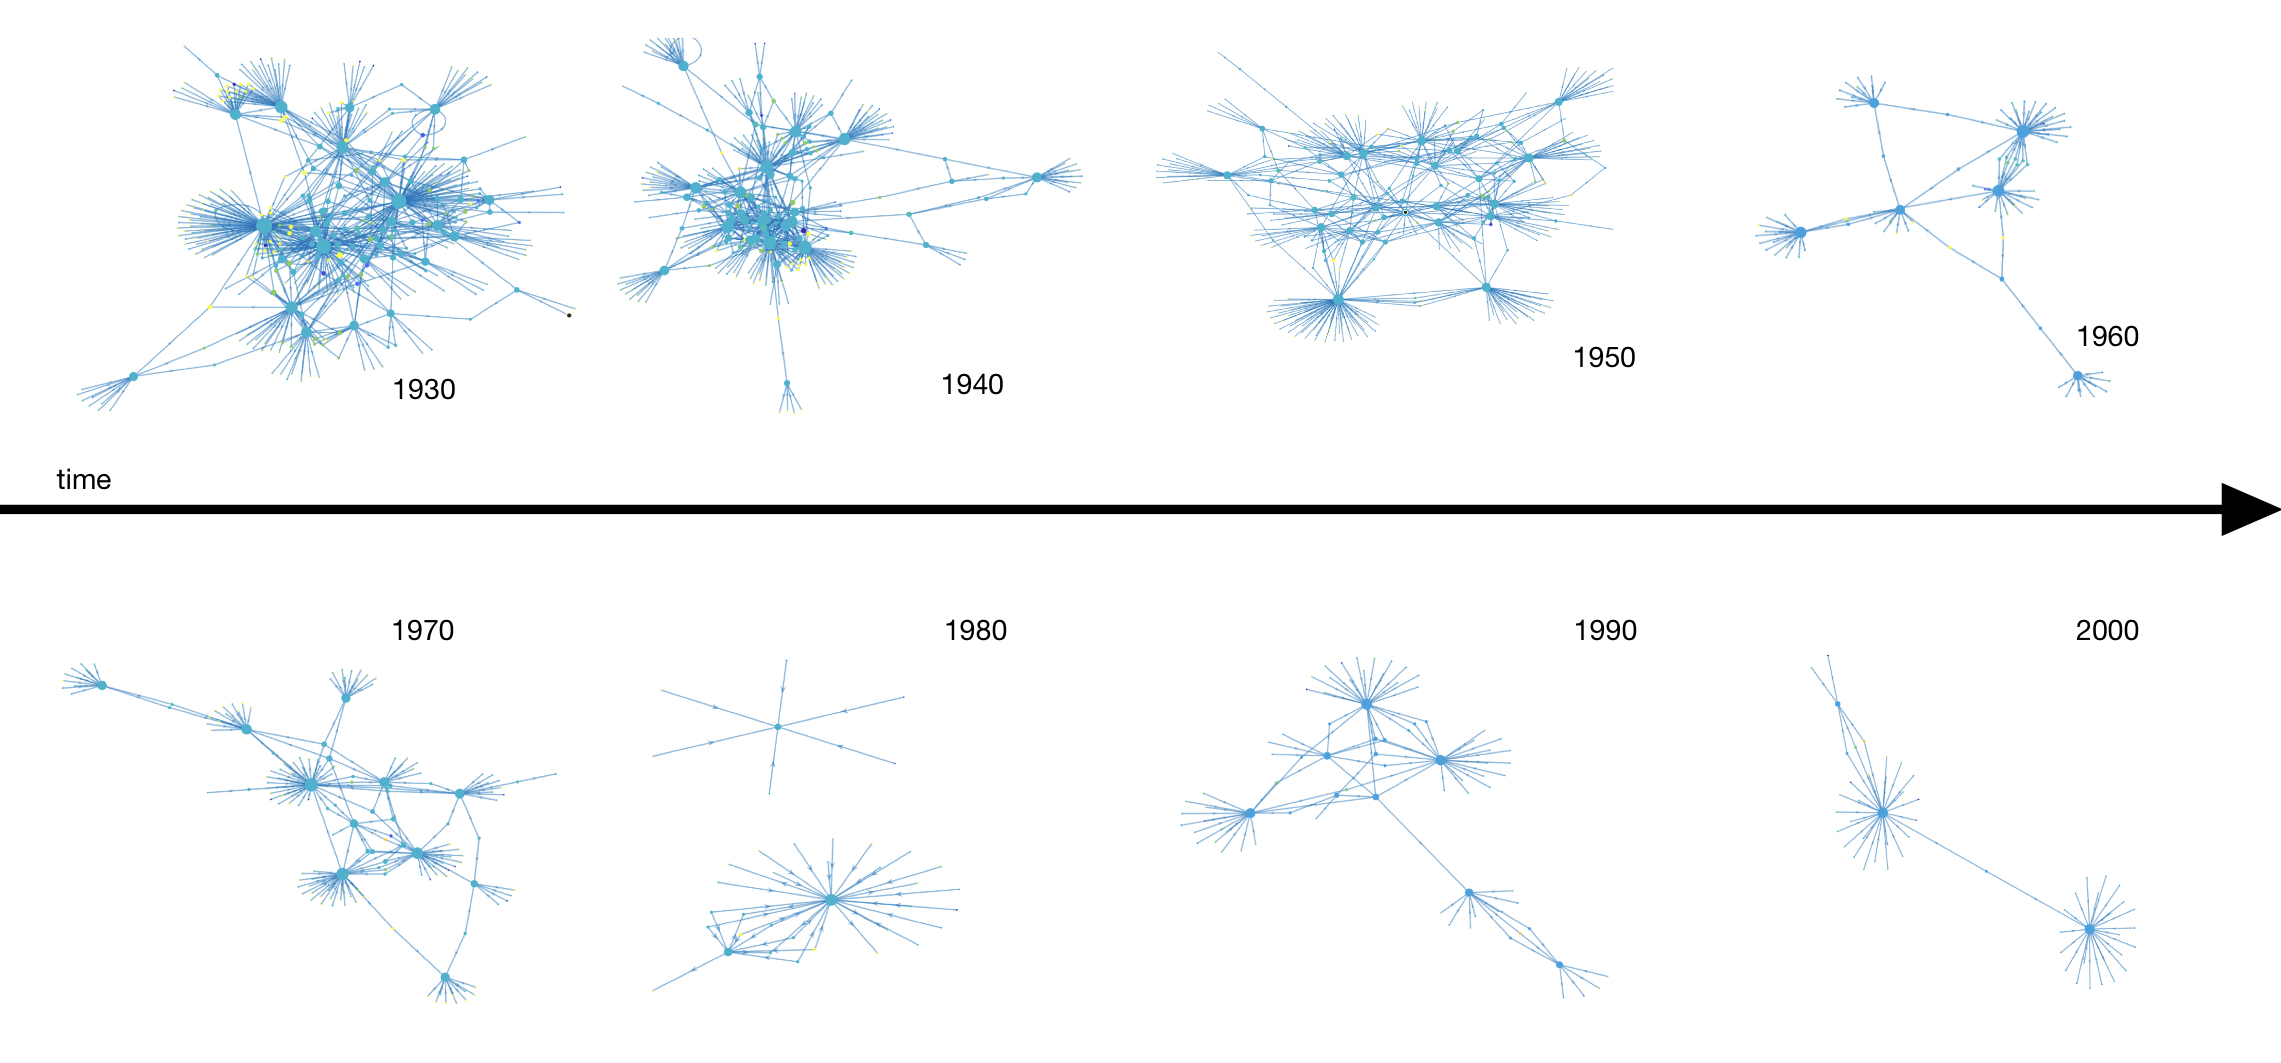
\includegraphics[width=8cm]{shijian.png}
		\caption{vocal-organization}
	\end{minipage}
	\begin{minipage}[t]{0.48\textwidth}
		\centering
		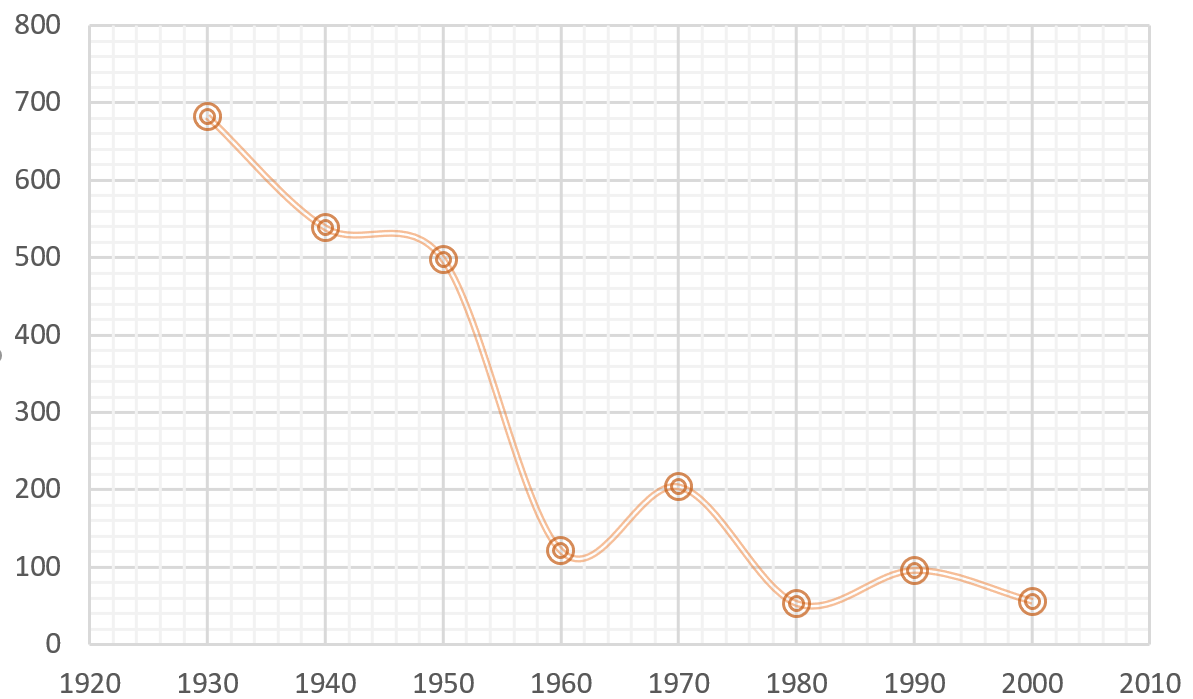
\includegraphics[width=7cm]{f of vocal.png}
		\caption{$\psi(t)$ of every year}
	\end{minipage}
\end{figure}


Obviously, we can see that after experiencing the glory of the 1930s, vocal gradually declined. In the 1970s and 1990s, vocal actively absorbed some characteristics of other schools, such as jazz and Pop. However, it can not avoid the gradual decline of this community.

\subsection{Analysis of specific factors}

Then, in order to explore the specific changes of the style of vocal school over time, we make statistics of the main changes in the data of vocal.

\begin{figure}[H]
    \centering
    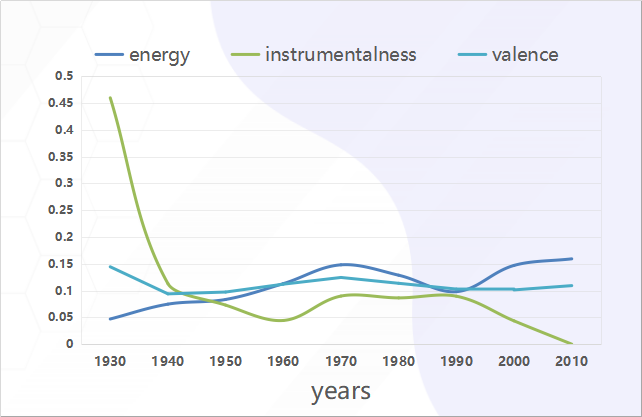
\includegraphics[width=.7\textwidth]{vocal.png}
    \caption{The main factors of style change}
    \label{img}
\end{figure}

In Task3, we summarized the main characteristics of each genre, where the Jazz genre is mainly characterized by the use of instruments, the Pop/Rock genre is mainly characterized by high energy attribute value, and the R\&B genre is mainly characterized by high valence attribute, which is more aggressive.

In the 1970s and 1980s, the Vocal genre was briefly influenced by the R\&B genre, but its valence values did not fluctuate significantly, so we can assume that the R\&B genre did not have much influence on the Vocal genre in terms of valence.

The influence of the Pop/Rock genre on the Vocal genre is obvious, as the Pop/Rock genre began to influence the Vocal genre from the 1950s onwards, and the value of the energy attribute of Vocal increased rapidly. By the 1980s, the Pop/Rock genre no longer influenced the Vocal genre, and Vocal's energy attribute values fell. In the 1990s, the Pop/Rock genre once again entered the ranks of influencers, and Vocal's energy attribute values began to climb again. Therefore, we can speculate that the characteristics of Vocal's energy were mainly influenced by the Pop/Rock genre.

\subsection{An analysis of the influence of artists}

In order to explore how artists are influenced with the passage of time, we select Frank Sinatra, the main character of vocal school, for specific analysis.

As a veteran artist who became famous in the 1920s, Frank Sinatra did not have many influences during his career. According to statistics, he was only influenced by the Vocal genre five times in the 1930s, the Jazz genre twice, and the Vocal genre once in the 1940s.

Based on the data of his career releases, the characteristics of his works were counted every ten years, and the fluctuating attributes of instrumentalness, liveness, and acousticness were plotted over time, as shown in the following graph:

\begin{figure}[H]
    \centering
    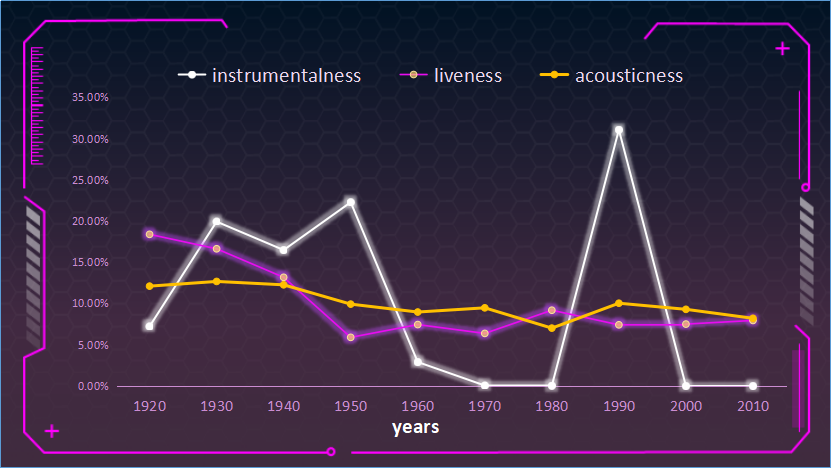
\includegraphics[width=.6\textwidth]{Frank.png}
    \caption{The main changes of Frank}
    \label{img}
\end{figure}

It is clear from the graph that Frank Sinatra's instrumental use improves significantly in the 1930s as he is influenced by two composers of the Jazz genre. He was then influenced by the Vocal genre in the 1940s, and the value of the instrumentalness attribute then slipped. The year-to-year decline in the liveness attribute is most likely due to the popularity of electronic playback technology, to the extent that his performances were more often transmitted via television. The spike in his instrumentalness attribute in the 1990s was likely influenced by the explosion of electronic music at the time.

\section{Task7: Other factors}
We make a curve of eigenvalues over time based on the data\_by\_year data and selected a few eigenvalues with large variance:

\begin{figure}[H]
	\centering
	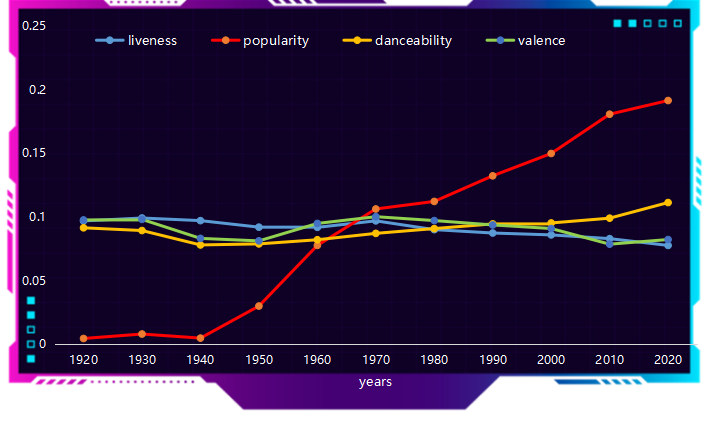
\includegraphics[width=.7\textwidth]{t71.png}
	\caption{The main changes of Frank}
	\label{img}
\end{figure}
We can explore the impact of fluctuations in the curve in the following ways:

\begin{itemize}
	\item \textbf{Impact of the World War II}
\end{itemize}

	In the 1940s, World War II broke out, and because the war had a melancholy color, the works created in the 1940s were also more negative (less valence) and less suitable for dance, resulting in less danceability. At the same time, Europe was caught in the middle of the war, and a large number of European artists immigrated to the United States for refuge. After World War II, the music artists who immigrated from Europe and the native American music artists influenced each other, which made the music develop well. Coupled with the relatively peaceful international environment after World War II, people had more energy and leisure time to enjoy music, and the popularity of music had a great development after World War II\upcite{3}
	.
	
\begin{itemize}
	\item \textbf{The impact of information technology}
\end{itemize}

	The emergence of the Internet in the 1970s and its subsequent development diversified the vehicles and media for disseminating musical works and made it cheaper and more convenient, and the popularity of music continued to increase. At the same time, however, offline musiac was more costly and therefore accounted for less than the ease and affordability of distributing music online, thus reducing the liveness characteristics of music.

\begin{itemize}
	\item \textbf{The impact of politics}
\end{itemize}

	During the anti-war and civil rights movements in the United States in the 1960s, rock and roll made a huge impact on mainstream culture as a powerful weapon for youth subculture groups. During these movements, rock music was loved by many people. The danceability of the music increased due to the passionate rhythm of rock and roll, which made people dance to the music involuntarily\upcite{4}

\begin{itemize}
	\item \textbf{The impact of the economy}
\end{itemize}

	In the 1930s, the economic crisis broke out across the United States, and the unemployment rate rose sharply in the face of closures and bankruptcies brought about by the Great Depression. The record industry at the time was hit hard. The music industry was hit hard and the popularity of music declined from the 1930s to the 1940s\upcite{5}
	
\section{Analysis on Model's Sensitivity}
In Task 1, we introduce the attenuation coefficient $\mathcal{P}$ and assign it a value of 0.5 in order to measure the effect of indirect influence in the influence network, and now we do a sensitivity test on the attenuation coefficient $\mathcal{P}$.
\begin{figure}[H]
	\centering
	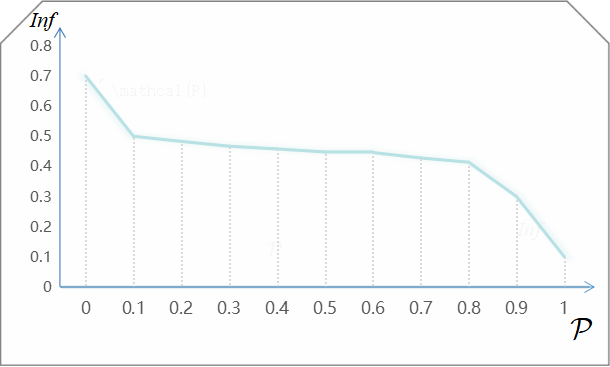
\includegraphics[width=.6\textwidth]{lingmin.png}
	\caption{The main changes of Frank}
	\label{img}
\end{figure}
From the figure we can find that there is no large change in the influence when $\mathcal{P}$ is taken at [0.1,0,8]. Therefore, our model is insensitive to $\mathcal{P}$ in most cases.

\section{Strengths and Weaknesses}
\begin{itemize}
\item Strengths:
\end{itemize}

1.It is innovative to construct influence models through networks.

2.The selection of the network parameters of the influence network is scientific and reasonable.

\begin{itemize}
\item Weaknessess:
\end{itemize}

1.Because of the large amount of data, our model cannot analyze each genre thoroughly.

2.The indicators of the popularization model cannot be quantified, resulting in a low persuasibility of the model.

3.As time changes, artists in one genre may create music in other genre styles, and we cannot consider this situation.

4.We did not consider the impact that a collaboration between artists would have on the work.
\newpage

% 以下为信件/备忘录部分,不需要可自行去掉
% 如有需要可将整个 letter 环境移动到文章开头或中间
% 请在后一个花括号内填写信件(Letter)或备忘录(Memorandum)标题
%审视艺术家和流派的进化和革命趋势
\begin{letter}{A document to the ICM Society}
	\begin{flushleft}  % 左对齐环境,无首行缩进
	To whom it may concern,
	\end{flushleft}

Music, as an essential component of cultural heritage, contains tremendous value.In order to measure musical influence and to explore the evolutionary and revolutionary trends in examining artists and genres, we build a network model.

Through our network model, we can identify the change-makers in the genre, such as the artist Joan Baez, who pushed the Folk genre to merge with the Jazz genre, and the artist The Beatles, who influenced not only the genre, but all other genres.

Unfortunately, however, due to the limited amount of data available, we only know the main genre of an artist and some of his works, while in reality, an artist does not belong to only one genre, but his works often dabble in multiple genres. And, in reality, there are fusions and divisions between genres. For example, the country genre can be subdivided into Bluegrass, Country Pop, Countrypolitan, etc. These factors also interfere with the accuracy of our model.

In addition, due to the lack of data, our model is unable to quantify the impact of environmental and major events on music. For example, we found that the Second World War around 1940s saw relatively large ups and downs in the characteristics of all music genres, but it is difficult to accurately reflect this factor in our model.

With this data, we can revise our network model, add influence factors in the network, and thus more accurately analyze the development and change of music genres.

Other factors will have an impact on the music, and likewise, the music will have an impact on other factors. For example, the rise of rock music in the United States in the 1950s elevated white Americans' identification with blacks, eased the problem of racial tension in the United States, and made the country more culturally inclusive.%此处引用

Music as a part of culture, while having a profound impact on the rest of culture. Music can not only be enjoyed, but it can also permeate social life. And this is where the value of music lies.

\hfill Yours Sincerely,

\hfill Team $\#$2107542  
\end{letter}

\clearpage
\begin{thebibliography}{99}
	\bibitem{1} Jianshu Weng, Ee-Peng Lim, Jing Jiang. TwitterRank: Finding Topic-sensitive Ibfluential Twitterers
	\bibitem{2} http://www.360doc.com/content/14/0505/10/15883912\_374732455.shtml.
	\bibitem{3} Wang Lei. The Post-World War II American Art Patronage System and the Rise of American Contemporary Art [D]. China Academy of Art, 2015.
	\bibitem{4}  Zhao Dongliang. The relationship between rock music and social movements in the United States in the 1960s[J]. Literary and Educational Materials,2018(6):94-95.
	\bibitem{5}Ding Zhu. The history of popular music (serialized five) [J]. Music Life,2011(07):28-29.
	\bibitem{6}YUNJING DAI. A Research of Quantification of Pairwise Influence in Online Social Network. 
	\bibitem{7}Yu Xin. Tradition in innovation: a glimpse of western music in the twentieth century.2006sk079
	\bibitem{8}Grout, A History of Western Music. People's Music Publishing House,1996, p. 720.
	\bibitem{9} Shen Xuan. A Brief History of Western Music. Shanghai Music Publishing House,1999, p. 319.
\end{thebibliography}

\end{document}  % 结束$
%http://www.360doc.com/content/14/0505/10/15883912_374732455.shtml
%Task5里的参考文献